\documentclass[11pt]{article}
\usepackage[utf8]{inputenc}
\usepackage[T1]{fontenc}
\usepackage{lmodern}
\usepackage[margin=1in]{geometry}
\usepackage{setspace}
\usepackage{amsmath,amssymb,amsthm,mathtools,bm}
\usepackage{booktabs,tabularx,multirow,threeparttable}
\usepackage{graphicx,caption,subcaption}
\usepackage{enumitem}
\usepackage[authoryear,round]{natbib}
\usepackage{xcolor}
\usepackage{url}
\usepackage[colorlinks=true,linkcolor=blue!50!black,citecolor=blue!50!black,urlcolor=blue!50!black]{hyperref}
\usepackage[nameinlink,capitalise]{cleveref}

\onehalfspacing
\setlist{itemsep=2pt,topsep=4pt}

\newtheorem{theorem}{Theorem}
\newtheorem{proposition}{Proposition}
\newtheorem{lemma}{Lemma}
\newtheorem{corollary}{Corollary}
\theoremstyle{definition}
\newtheorem{assumption}{Assumption}
\newtheorem{definition}{Definition}
\theoremstyle{remark}
\newtheorem{remark}{Remark}
\crefname{assumption}{Assumption}{Assumptions}

\newcommand{\E}{\mathbb{E}}
\newcommand{\R}{\mathbb{R}}
\newcommand{\Phat}{\hat P}
\newcommand{\Pbar}{\bar P}
\newcommand{\vhat}{\hat v}
\newcommand{\eps}{\varepsilon}
\newcommand{\dd}{\mathrm{d}}
% Generated by code/scripts/make_figures.py -- do not edit by hand.
\newcommand{\calPhat}{23}
\newcommand{\calPm}{12.0}
\newcommand{\calvhat}{2.13}
\newcommand{\calF}{1.772}
\newcommand{\calT}{1.7}
\newcommand{\calPremium}{18\%}
\newcommand{\calRent}{20\%}
\newcommand{\calGainPeak}{17\%}
\newcommand{\calDissip}{17\%}
\newcommand{\calPlannerGain}{4.4\%}
\newcommand{\calSubsidy}{4.4\%}
\newcommand{\calGstar}{20\%}
\newcommand{\calEta}{0.033}
\newcommand{\calLambda}{0.975}
\newcommand{\calEpsW}{0.125}
\newcommand{\calLambdaLo}{0.966}
\newcommand{\calLambdaHi}{0.995}
\newcommand{\calEpsV}{0.043}
\newcommand{\calBeyond}{11\%}
\newcommand{\calZhat}{0.80}
\newcommand{\calLin}{5.5\%}
\newcommand{\calQone}{$-9.1$\%}
\newcommand{\calQfour}{$+2.1$\%}
\newcommand{\calQfive}{$+3.9$\%}
\newcommand{\calWQfour}{$+1.0$\%}
\newcommand{\calWQfive}{$+1.2$\%}
\newcommand{\calXm}{0.91}
\newcommand{\calCoverage}{0.72}
\newcommand{\calPhi}{0.67}
\newcommand{\calAware}{39\%}
\newcommand{\calErosion}{2.0\%}
\newcommand{\calShareGrowth}{27\%}
\newcommand{\calShareCons}{20\%}
\newcommand{\calShareMature}{53\%}
\newcommand{\calWriteOut}{25.6}
\newcommand{\calReadDens}{14.1}
\newcommand{\calReadOut}{0.54}
\newcommand{\calCatchDens}{65.3}
\newcommand{\calCatchGstar}{22.4}

% Generated by empirics/12_tables.py -- do not edit by hand.
\newcommand{\empRDtopfive}{0.69}
\newcommand{\empRDtopfiveBefore}{0.30}
\newcommand{\empRDcitesIns}{$-0.137$}
\newcommand{\empRDcitesInsSE}{0.060}
\newcommand{\empRDprior}{$-0.051$}
\newcommand{\empRDpriorSE}{0.017}
\newcommand{\empRankN}{87{,}694}
\newcommand{\empRankSD}{0.45}
\newcommand{\empRankCites}{0.023}
\newcommand{\empRankCitesSE}{0.016}
\newcommand{\empRankCitesMain}{0.031}
\newcommand{\empRankCitesMainSE}{0.018}
\newcommand{\empRankUsevfive}{$-0.0049$}
\newcommand{\empRankUsevfiveSE}{0.0038}
\newcommand{\empRankUsevfiveMean}{0.068}
\newcommand{\empRankUsevfiveUB}{3.9\%}
\newcommand{\empRankUsevfiveMDE}{16\%}
\newcommand{\empRankAsevfive}{$-0.0001$}
\newcommand{\empRankAsevfiveSE}{0.0041}
\newcommand{\empRankSelf}{$-0.048$}
\newcommand{\empRankSelfSE}{0.015}
\newcommand{\empAwareInsFifty}{34\%}
\newcommand{\empAwareInsSevfive}{50\%}
\newcommand{\empAwareInsNinety}{61\%}
\newcommand{\empSelfShare}{50\%}
\newcommand{\empEndMath}{2.4}
\newcommand{\empEndMathSE}{0.3}
\newcommand{\empEndOther}{3.4}
\newcommand{\empEndOtherSE}{0.3}
\newcommand{\empEndStag}{1.7}
\newcommand{\empEndStagSE}{0.4}
\newcommand{\empEndOtherRel}{15\%}
\newcommand{\empEndMathRel}{17\%}
\newcommand{\empEndNoTrackOtherRel}{17\%}
\newcommand{\empCSdid}{1.32}
\newcommand{\empCSdidSE}{0.10}
\newcommand{\empCSpre}{2.7}
\newcommand{\empCSpost}{1.3}
\newcommand{\empCSperMonthPre}{290}
\newcommand{\empCSperMonthPost}{187}
\newcommand{\empCSdoseFS}{0.41}
\newcommand{\empCSdoseFSSE}{0.10}
\newcommand{\empCSdoseRF}{$-0.70$}
\newcommand{\empCSdoseRFSE}{0.26}
\newcommand{\empCSdoseRFpl}{$-0.32$}
\newcommand{\empCSdoseRFplSE}{0.17}
\newcommand{\empCapPre}{1.66\%}
\newcommand{\empCapOct}{0.38\%}
\newcommand{\empCapRemoved}{1.3\%}
\newcommand{\empCapVol}{0.220}
\newcommand{\empCapVolPrev}{0.175}
\newcommand{\empLLMall}{0.022}
\newcommand{\empLLMallSE}{0.005}
\newcommand{\empLLMnonai}{0.024}
\newcommand{\empLLMnonaiSE}{0.007}
\newcommand{\empLLMallPct}{7\%}
\newcommand{\empLLMn}{68{,}467}
\newcommand{\empLLMadopters}{4{,}488}
\newcommand{\empLLMpre}{0.039}
\newcommand{\empRDcitesSS}{$-0.175$}
\newcommand{\empRDcitesSSSE}{0.032}
\newcommand{\empRDcitesSSN}{43{,}097}


\title{Too Fast to Read:\\Topic Choice and the Incidence of Research Tools}
\author{}
\date{October 2026}

\begin{document}
\maketitle

\begin{abstract}
\noindent Reading has two jobs in science. It \emph{teaches}, raising the quality of new work, and it \emph{protects}, revealing projects that others have already done. We model researchers who choose a topic, split their time between producing and reading, and must read a topic's literature before they can join it. For any learning and detection technology with bounded absorption, the payoff of working in a topic is single peaked in the flow of its literature, and free choice of topics has the structure of a system of cities. Two results follow. First, a speed limit: no newcomer can catch up with a literature that grows faster than she reads, so such topics close, rents near the limit grow without bound, fast-growing topics overshoot and slow ones never take off. Second, frontier incidence: output per researcher equals the value of opening a new topic, so a research tool is worth what it adds to that value. Inside a topic every speed-up is worth the same per hour saved; entry ranks them. Production tools survive almost fully; reading tools survive mainly through founders who stay in the topics they open, and catch-up tools least. Valued by readership rather than credit, the ranking reverses. On arXiv, more volume opens new ground rather than thickening old topics. On 2.2 million submissions with exact timestamps, four arXiv rule changes and design features identify the margins the model relies on. A tighter endorsement rule cut first-time submitters by about a sixth. A peer-review requirement halved review articles in computer science. A cap of two submissions per person per month binds on about one paper in a hundred. Daily listing position barely moves readership and leaves the detection of overlapping work unchanged. In the calibrated model, per hour saved, a production tool is worth \calPerHour--\calPerHourNoF\ times a reading tool, and the static gain from optimal topic choice is small.

\medskip
\noindent\textbf{JEL:} O31, O33, O40, D62, I23, R12. \quad \textbf{Keywords:} economics of science, topic choice, duplication, system of cities, burden of knowledge, incidence, artificial intelligence, arXiv.
\end{abstract}

\newpage
\section{Introduction}\label{sec:intro}

Submissions to arXiv more than doubled between 2018 and 2025, and in September
2026 the archive received a record 40,363 papers. Large language models now
draft text faster than any researcher can, and they are starting to read and
summarise for us too. Two opposite hopes and fears follow. Faster writing
might flood science with duplicates. Better reading tools might be the remedy
and raise research productivity. This paper argues that free choice of
research topics turns both intuitions around. Faster writing scales science,
while better reading tools are largely competed away.

The argument rests on one observation: researchers choose not only how much to
read and write but \emph{where} to work. Reading has two jobs. It
\emph{teaches}: what one reads raises the quality of one's own work, and more so
in a topic with more to learn from. It \emph{protects}: each earlier paper may
already cover one's project, and reading is how one finds out. Unaware
duplicates lose part of their credit; detected overlaps can be turned into
follow-ons that cite the earlier work, or abandoned. These two jobs make the
payoff of working in a topic rise with the flow of its literature while there is
much to learn, and fall once more of that flow goes unread. Newcomers enter
topics until they are no better than the frontier, where new topics are opened.

\paragraph{The headline result.} A tool that speeds up writing raises the payoff
of everything a researcher does, including opening a new topic. Newcomers spread
out, so output per researcher rises almost one for one with writing speed, and
the duplication rate barely moves (\cref{prop:ai,prop:solow}). A tool that
speeds up reading, search or catching up on a literature raises the payoff only
of working inside existing topics. Newcomers crowd in until those topics are
again no better than the frontier. Density rises, fewer topics are opened, and
output per researcher rises only to the extent that the frontier improves as
fewer directions are taken. The gain from better reading is dissipated by entry
in the same way that a better road into a city is capitalised into its size.
This asymmetry gives one reason why decades of better access to the literature
have coincided with falling measured research productivity
\citep{bloometal2020}.

\paragraph{What is new, and what is not.} The equilibrium structure is that of
a system of cities \citep{henderson1974} or of clubs \citep{buchanan1965}. The
average payoff is single peaked in group size, new groups enter freely,
equilibria are stable only on the falling side, the planner sits at the peak
of the average payoff, and an entry tax decentralises the optimum. Self-organised
cities are too large for the same reason \citep{hendersonbecker2000,scotchmer2002}.
We use this structure and claim four things that it does not provide. First,
a microfoundation of the hump in the two jobs of reading, valid for any
learning and detection technology in a broad class. The proof uses joint
log-concavity of the researcher's problem in reading time and density
(\cref{thm:v}), and the hump comes from bounded absorption against a covering
hazard that grows with the literature. Second, the crowders are the readers:
the sign of the spillover from one more paper is derived from the envelope
theorem rather than assumed, and it changes along the payoff curve
(\cref{prop:externality}). Third, the duplication rate is pinned by entry, with
an exact volume elasticity of density built from observables
(\cref{prop:volume}). Fourth, the writing--reading asymmetry, together with a
sufficient statistic for the stepping-on-toes parameter of growth theory
(\cref{prop:sot}). A catch-up cost, the need to read a topic's stock before
contributing \citep{jones2009}, adds a wedge that the city literature lacks:
incumbents' returns rise with density even where newcomers find topics too
crowded (\cref{cor:overcrowd}).

\paragraph{Evidence.} We confront the model with the arXiv record in two ways.
The descriptive evidence (\cref{sec:facts}) comes from 1.49 million papers posted
in 2018--2025, classified into 150 text-based areas. The anchor fact is that volume
opens new ground. From the 95th to the 25th percentile similarity radius, local
density rises with area volume at an elasticity of 0.12--0.19, against 0.53--0.81
if papers kept landing in the same idea space. At the closest-overlap radius the
estimate is 0.035, though it is imprecise (SE 0.118). Returns are hump-shaped in
topic density. Unaware duplicates lose about a fifth of their citations, close to
the 21\% penalty for scooped teams in \citet{hillstein2025}, while aware
follow-ons gain. Once corrected for citation recall, about 60\% of close overlap
is aware.

The quasi-experimental evidence (\cref{sec:causal}) uses arXiv's own rules on a
new panel of 2.2 million arXiv submissions with exact timestamps through
15~October 2026. Four shocks speak to the margins the model relies on.
\begin{itemize}
\item \emph{Entry cost.} In January 2026, arXiv stopped endorsing new submitters
on the strength of an institutional e-mail address alone; Mathematics had moved
in December 2025. The share of papers by first-time submitters fell by
\empEndOther\ percentage points (about \empEndOtherRel) in the affected
sections, net of the year before. The staggered timing matches the rule.
\item \emph{Catch-up cost.} From November 2025, review and position papers in
computer science needed prior peer review. Review-type papers in computer
science halved relative to other archives, more so in categories that had
relied on them. First-time authorship fell more in those categories, though a
smaller pre-trend of the same sign makes this suggestive.
\item \emph{Writing cap.} From October 2026, each person may submit at most two
papers a month. The cap removed about \empCapRemoved\ of papers. Total volume
kept growing at its usual seasonal pace, so per-submitter caps are a weak lever
on volume.
\item \emph{Readership.} A paper's position in the daily listing depends on how
many others submitted earlier that day. We use this to test the
detection channel directly. Position has only a small effect on citations, and
no detectable effect on later overlapping work or on the share of it that cites
the paper, with tight bounds. Overlap is detected by targeted search rather than
by browsing.
\end{itemize}
At the author level, adopters of LLM-style writing raised their output by about
\empLLMallPct\ relative to non-adopters. That is far less than the 36\% of
\citet{kusumegietal2025}, whose design has been criticised for mechanically
generating positive dynamics \citep{renaultetal2026}.

\paragraph{Magnitudes.} The calibrated model is disciplined by the corrected
arXiv moments (\cref{sec:quant}). The reading--writing asymmetry is the
quantitatively robust prediction: a 30\% faster pen raises output per researcher
by \calWriteOut\ log points, while 30\% faster reading raises it by only
\calReadOut. The static welfare cost of crowding is small. Optimal topic choice
would raise output per researcher by \calPlannerGain\ in the baseline calibration
and \calWPlannerGain\ in the within-topic one, and overlap destroys only about
\calErosion\ of credit at mature density. The frictionless benchmark, in which
catch-up is free and topics fill until the whole rent at the peak is dissipated,
would lose \calDissip; it is a counterfactual, not the calibrated economy. The
direction of the inefficiency survives treating all priority credit lost to
overlap as a transfer between racers (\cref{prop:social}). With the measured
volume elasticity, topic crowding explains little of the decline in research
productivity.

\paragraph{Implications.} Two further results follow, and we collect them in
\cref{sec:macro}. Because the stock of literature lags its flow, topics whose
literature grows faster than a threshold rate overshoot their best density.
This survives forward-looking entry: rational entrants overshoot more than
myopic ones once a topic grows fast, because what deters entry is the stock,
and a young topic has little of it (\cref{prop:toofast}). And the
stepping-on-toes parameter equals one minus the product of the volume
elasticity of density and the slope of the entrant's payoff curve.

\paragraph{Related literature.} The paper joins five literatures. The first is
the economics of science and priority
\citep{merton1957,merton1961,dasguptadavid1994,stephan1996,hillstein2025,hillstein2025race,bobtcheffetal2017}
and the philosophy of the division of cognitive labour
\citep{kitcher1990,strevens2003}. We add reading as a choice with two
distinct roles, and derive rather than assume the costs of duplication.
\citet{hillstein2025race} show that priority races lower quality; our cost of
crowding works through detection and catch-up instead, and the two are
complementary. The second is the theory of excess entry, common pools, cities and
clubs
\citep{gordon1954,weitzman1974,mankiwwhinston1986,henderson1974,buchanan1965,hendersonbecker2000,scotchmer2002}
and of patent races \citep{loury1979,dasguptastiglitz1980}. Our resource is
attention to a literature, and the crowders are its readers. The third is the
direction of research
\citep{bryanlemus2017,hopenhaynsquintani2021,carnehlschneider2025,bramoullesaintpaul2010,rzhetskyetal2015,fosteretal2015,myers2020,borjasdoran2012,borjasdoran2015,azoulayetal2019}.
\citet{carnehlschneider2025} model the choice of question by novelty and
feasibility. We model the choice by density, derive the hump, and measure the
margin. \citet{borjasdoran2015} document that researchers move in idea space in
response to crowding, which is the margin our model turns on. The fourth is the
macroeconomics of ideas and of access to knowledge
\citep{romer1990,aghionhowitt1992,jones1995,kortum1997,weitzman1998,bloometal2020,jones2009,ekerdtwu2024,furmanstern2011,murrayetal2016,iariaetal2018,biasimoser2021,evans2008,mccabesnyder2015,agrawaletal2016,parketal2023}.
We give stepping on toes an equilibrium foundation and explain why better access
to the literature need not raise productivity. The fifth is artificial
intelligence in science
\citep{agrawaletal2019,brynjolfssonetal2019,jones2025ai,duedeetal2026,haoetal2026,liangetal2024,kusumegietal2025}.
\citet{jones2025ai} studies AI in a task-based R\&D production function, and
\citet{duedeetal2026} model LLMs as labour-augmenting technology that shifts
effort across projects. We separate writing, entry, reading, search and catch-up
channels by their equilibrium footprints. Methodologically, our text-based
density measures follow \citet{hobergphillips2016} and \citet{kellyetal2021}, and
the listing-position design builds on \citet{haqueginsparg2009,haqueginsparg2010}
and \citet{feenbergetal2017}.

\Cref{sec:model} sets up the model and \cref{sec:payoff} derives the payoff
curve. \Cref{sec:frictionless,sec:catchup} characterise equilibrium, welfare and
social value. \Cref{sec:ai} states the writing--reading asymmetry.
\Cref{sec:facts,sec:causal} present the descriptive and quasi-experimental
evidence, \cref{sec:quant} quantifies the model, \cref{sec:macro} collects
the implications for fast-growing topics and growth, \cref{sec:predictions}
lists out-of-sample predictions, and \cref{sec:conclusion} concludes.

\section{Model}\label{sec:model}

The economy is stationary. Time is continuous, but within a topic the relevant
literature is a flow, so we describe a researcher's choices per unit of time.

\subsection{Researchers, topics and time}

There is a continuum of topics. Topics that are open are ex ante identical. A
mass $N$ of researchers each has one unit of time per period, split into a
share $x$ spent writing and a share $r=1-x$ spent reading. Writing full time
yields $a$ papers (projects) per period. Topic $j$ hosts $n_j$ researchers who
write, and receives a flow of
\begin{equation}\label{eq:flow}
P_j = a\,x\,n_j
\end{equation}
papers per period. $P_j$ is the topic's \emph{density}. We call the ratio of
writing speed to reading speed, $a/b$, the \emph{pace} of science.

\subsection{Reading teaches}

A researcher who reads full time reads $b$ papers per period, so a reading
share $r$ yields $R=b\,r$ papers drawn from her topic's flow. What she reads
raises the quality of her own work by the factor $Q(R,P)$.

\begin{assumption}[Learning]\label{ass:Q}
$Q:\R_+^2\to[1,\infty)$ is continuous, twice continuously differentiable on
$\R_{++}^2$, nondecreasing in both arguments, with $Q(0,P)=Q(R,0)=1$ and
$\bar Q(R)\equiv\sup_P Q(R,P)<\infty$ for every $R$. Moreover $\ln Q$ is
jointly concave and supermodular on $\R_+^2$.
\end{assumption}

Nothing is learned without reading or without a literature to read, and what
one can learn is bounded by what one reads. Concavity of $\ln Q$ rules out
increasing returns to reading. Supermodularity says that reading is worth
more in a topic with more to learn from. Our running example is
\begin{equation}\label{eq:Qexample}
Q(R,P) = \big(1+\beta\,h(R,P)\big)^{\gamma},\qquad h(R,P)=\frac{RP}{R+P},\qquad \beta>0,\;\gamma\in(0,1].
\end{equation}
The harmonic aggregator $h$ is close to $R$ when the reader samples a small
part of a rich literature and close to $P$ when she reads a thin literature
exhaustively. Because $h$ is concave and homogeneous of degree one, the
example satisfies \cref{ass:Q} (\cref{app:proofs}).

\subsection{Reading protects}

Each paper in the flow \emph{covers} a given project independently with a small
probability. The number of covering papers is therefore
Poisson with mean $\theta P$. A covering paper is caught only if it is read. With reading
coverage $c=R/P$ it is caught with probability $\varphi(c)$.

\begin{assumption}[Detection]\label{ass:phi}
$\varphi:\R_+\to[0,1]$ is continuous and twice differentiable on $(0,\infty)$,
with $\varphi(0)=0$, $\varphi'>0$ and $\varphi''<0$.
\end{assumption}

Concavity says that the first papers one reads are the most informative about
overlap. Random reading with replacement gives $\varphi(c)=1-e^{-c}$. Our
example $\varphi(c)=1-e^{-\sigma c}$ indexes \emph{search precision} by
$\sigma$: a better search engine finds covering papers sooner.

\paragraph{Credit.} Overlap erodes credit multiplicatively. Each covering paper
that goes unread turns part of the project into a duplicate and removes a
share $\lambda$ of its credit. When a covering paper is caught, the
researcher chooses between two options. She can \emph{pivot} to a fresh variant at a time cost
that leaves a share $1-\kappa_p$. Or she can \emph{proceed} as a follow-on
that cites the earlier paper and keeps a share $\delta$ drawn from a
distribution $G$. She proceeds if $\delta>1-\kappa_p$. The expected share kept
after a detection is $1-\ell\equiv\E\max\{\delta,1-\kappa_p\}$.

\begin{assumption}[Credit]\label{ass:credit}
$0\le \ell<\lambda\le 1$ and $\theta>0$.
\end{assumption}

Detection is valuable ($\ell<\lambda$), and duplicates need not earn zero
($\lambda<1$ is allowed). The arXiv evidence (Fact~\ref{fact:credit}) requires
both. Credit here is private. \Cref{sec:catchup} separates it from social
value, since part of the credit lost to overlap may be a transfer to the
earlier paper. Let $\Delta\equiv\lambda-\ell$ and $q\equiv 1-G(1-\kappa_p)$, the share
of detections that proceed.

\begin{lemma}[Credit and overlap]\label{lem:credit}
Under \cref{ass:phi,ass:credit}, expected credit per project is
\begin{equation}\label{eq:credit}
C(R,P)=\exp\!\Big\{-\theta P\big[\lambda-\Delta\,\varphi(R/P)\big]\Big\}.
\end{equation}
Covering papers that the researcher does not pivot away from (\emph{flagged
overlap}) arrive at rate $\theta P\,[1-(1-q)\varphi]$. A share
\begin{equation}\label{eq:aware}
A=\frac{q\,\varphi}{1-(1-q)\,\varphi}
\end{equation}
of them is \emph{aware}: the later paper cites the earlier one. Unaware
duplicates keep a share $1-\lambda$ of credit. Aware follow-ons keep
$\E[\delta\mid\delta>1-\kappa_p]$, which can exceed one.
\end{lemma}

The lemma follows from Poisson thinning. Detected and undetected covering
papers are independent Poisson counts with means $\theta P\varphi$ and
$\theta P(1-\varphi)$, and $\E[t^K]=e^{-\mu(1-t)}$ for $K\sim$ Poisson$(\mu)$.
Three features matter below. Only $\theta\lambda$ and $\Delta/\lambda$ enter
payoffs. Aware follow-ons are selected on high $\delta$, which is why they can
out-earn comparable papers. And the measured overlap flag is a fixed share of
covering events. Its level is a normalisation; its changes are not.

\subsection{The researcher's problem}

A researcher in a topic of density $P$ earns credit $a\,x\,Q(R,P)\,C(R,P)$ per
period. Writing $x$ projects is worth $x$, and each is worth $QC$. Dividing
by the common factor $a$,
\begin{equation}\label{eq:g}
g(r,P)\equiv(1-r)\,Q(br,P)\,C(br,P),\qquad v(P)\equiv\max_{r\in[0,1)}g(r,P).
\end{equation}
The \emph{payoff curve} $v$ is the central object of the paper. Writing speed $a$
scales every payoff and so drops out of $v$. The researcher takes $P$ as given:
she ignores both that her papers teach her colleagues and that they add to
what her colleagues must read.

\begin{remark}[Topic size and what density measures]\label{rem:breadth}
A topic has a fixed set of projects: the coverage rate $\theta$ is a property
of the topic and does not shrink when the topic attracts more people. This is
a normalisation, not a restriction, once density is measured locally. Let a
field of breadth $B$ consist of $B$ cells of unit breadth, each receiving a
flow $P/B$, and let researchers read and be covered within their own cell, so
that the coverage rate per paper is $\theta_0/B$. The field is then $B$
independent copies of a unit topic with density $P/B$, and every result below
holds with $P$ replaced by $P/B$. The model's topic is therefore a
neighbourhood of fixed size in idea space, and $P$ is papers per unit of idea
space: the quantity that nearest-neighbour similarity measures. If papers fall
at rate $P/B$ in a $d$-dimensional space, the distance to the $k$-th nearest
earlier paper scales as $(kB/P)^{1/d}$. ``Opening a topic'' means moving into
an empty cell, and the question of whether topics broaden as they grow becomes
the question of how the volume elasticity varies with the similarity radius,
which \cref{sec:facts} measures.
\end{remark}

\subsection{The frontier, careers and catch-up}

\paragraph{Frontier.} Instead of joining an open topic, a researcher may explore
new ground. An explorer opens a viable topic with probability $\pi(M)$, where $M$
is the measure of topics already open. If she succeeds, her output is worth
$f_0$ per unit of writing speed: the founding papers of a field. The frontier
pays $a\,F(M)$ in expectation, with $F(M)=f_0\,\pi(M)$. We assume $\pi$ is
continuous, positive and nonincreasing, with elasticity
$\eta\equiv -M\pi'(M)/\pi(M)\ge 0$: as more directions are taken, a fruitful
new one is harder to find \citep{kortum1997,bloometal2020}. Opening $M$ topics
takes $\Phi(M)=\int_0^M \dd m/\pi(m)$ researchers. We assume $F(M)<\vhat$, the
peak of the payoff curve defined below, so open topics are worth joining. A
newly opened topic attracts followers only if a thin topic beats the frontier,
$F<v(P_0)$, where $P_0$ is the flow of a newborn topic.

\paragraph{Careers and catch-up.} Researchers leave their topic at rate $\rho$
(retirement, a change of field) and are replaced by newcomers who choose a
topic. The literature a newcomer must master is a stock $S$ that accumulates
the flow and loses relevance at rate $\delta$: $\dot S=P-\delta S$, so
$S=P/\delta$ in a stationary topic. A newcomer must read it at speed $b_c$
before contributing. This is the \emph{catch-up} cost: a topic-level version
of the burden of knowledge of \citet{jones2009}. Explorers face no stock.

\begin{lemma}[Career value]\label{lem:career}
With exponential careers, a newcomer who joins a stationary topic of density
$P$ and then earns $a\,v(P)$ per period obtains, relative to an explorer, the
expected career value $w(P)/F(M)$, where
\begin{equation}\label{eq:w}
w(P)\equiv v(P)\,e^{-\kappa P},\qquad \kappa\equiv\frac{\rho}{\delta\, b_c}.
\end{equation}
In a stationary topic a share $1-e^{-\kappa P}$ of members are catching up,
so $w(P)$ is also output per member and the topic has
$n(P)=P\,e^{\kappa P}/(a\,x^\ast(P))$ members, where $x^*(P)$ is the optimal
writing share.
\end{lemma}

Catch-up takes $T=S/b_c=P/(\delta b_c)$ periods, and a career survives it with
probability $e^{-\rho T}=e^{-\kappa P}$. The frictionless benchmark is
$\kappa=0$ ($b_c\to\infty$). Incumbents earn $a\,v(P)$ per period;
newcomers earn $a\,w(P)$ on average over their careers.

\begin{table}[t]
\centering\footnotesize
\caption{Notation}\label{tab:notation}
\begin{tabularx}{\textwidth}{@{}>{\raggedright\arraybackslash}p{2.3cm}X@{\hspace{1.2em}}>{\raggedright\arraybackslash}p{2.1cm}X@{}}
\toprule
$a$, $b$ & papers written / read per period at full time & $P$ & topic density (flow of papers per period) \\
$x$, $r$ & writing and reading shares, $r=1-x$ & $R=br$, $c=R/P$ & papers read; reading coverage \\
$Q(R,P)$ & quality gain from what is read & $\varphi(c)$ & probability a covering paper is caught \\
$\theta$ & coverage rate per earlier paper & $\lambda$, $\ell$ & credit lost per unread / caught covering paper \\
$g(r,P)$, $v(P)$ & payoff per unit of $a$; its maximum & $\Phat$, $\vhat$ & peak of $v$ and its height \\
$F(M)$, $\pi(M)$ & frontier payoff; explorer's success probability & $\eta$ & elasticity of $\pi$ in topics opened $M$ \\
$\rho$, $\delta$ & career turnover; decay of the stock's relevance & $S$, $b_c$ & stock of literature; catch-up reading speed \\
$\kappa=\rho/(\delta b_c)$ & catch-up cost per unit of density & $w(P)$ & newcomer's career payoff, $v(P)e^{-\kappa P}$ \\
$P^*$, $P^m$ & equilibrium (mature) density & $\mathcal E$ & elasticity of density with respect to $N$ \\
$g$, $g^*$ & topic diffusion rate; overshooting threshold & $\lambda_J$ & stepping-on-toes parameter of \citet{jones1995} \\
$\lambda_s$, $\tau$ & social loss per unread covering paper; transfer share & $U(P)$ & entrant's expected payoff along the consolidation path \\
\bottomrule
\end{tabularx}
\end{table}

\subsection{Equilibrium}

\begin{definition}[Topic equilibrium]\label{def:eq}
A stationary topic equilibrium is a density $P^*$ for every open topic,
a writing share $x^*$ and a measure $M^*$ of open topics such that:
(i) $x^*=x^*(P^*)$ solves \eqref{eq:g};
(ii) newcomers are indifferent between joining any open topic and exploring:
$w(P^*)=F(M^*)$;
(iii) the allocation is stable under entry: $w'(P^*)<0$;
(iv) researchers add up: $\Phi(M^*)+M^*n(P^*)=N$.
\end{definition}

Condition (iii) selects allocations that survive the adjustment
$\dot n_j\propto w(P_j)-F(M)$. At a crossing where $w$ rises, one more entrant
raises the payoff of entering and draws in more. Topics in equilibrium need
not have the same density a priori, but (ii) and (iii) leave a single
admissible density, so they do. We state results in the \emph{large-topic
limit} $\Phi(M)/N\to 0$. Here topics are large relative to the researcher time
needed to open one, as they are in the data, where pioneers are a small share
of authors. \Cref{app:proofs} gives the general expressions.

\section{The payoff curve}\label{sec:payoff}

Every result in the paper rests on the shape of $v$. The next theorem shows
that it is single peaked for every learning and detection technology that
satisfies \cref{ass:Q,ass:phi,ass:credit}.

\begin{assumption}[Interior reading and learning potential]\label{ass:interior}
(a) Reading the first paper is worth its time: $b\,[\partial_R\ln Q(0,P)+\theta\Delta\varphi'(0)]>1$ for all $P>0$.
(b) A thin literature is worth reading: for some $\varrho>0$,
\[
\nu_0(\varrho)\equiv\lim_{P\downarrow 0}\frac{Q(\varrho P,P)-1}{P}-\frac{\varrho}{b}-\theta\big[\lambda-\Delta\varphi(\varrho)\big]-\theta_c\lambda_c>0.
\]
\end{assumption}

Part (b) compares, at the first papers of a topic, the gain from learning along
the ray $R=\varrho P$ with the time spent reading and the overlap risk. In the
example it reads $\sup_\varrho\{\gamma\beta\varrho/(1+\varrho)-\varrho/b-\theta[\lambda-\Delta(1-e^{-\sigma\varrho})]\}>\theta_c\lambda_c$.

\begin{theorem}[The payoff curve]\label{thm:v}
Under \cref{ass:Q,ass:phi,ass:credit}:
\begin{enumerate}[label=(\roman*)]
\item $v$ is continuous on $\R_+$, $v(0)=1$, $v(P)\ge e^{-(\theta\lambda+\theta_c\lambda_c)P}>0$ and $\lim_{P\to\infty}v(P)=0$.
\item $\ln v$ is concave on $(0,\infty)$. Under \cref{ass:interior}(a) it is strictly concave.
\item Under \cref{ass:interior}, there is a unique $\Phat\in(0,\infty)$ such that $v$ is strictly increasing on $[0,\Phat]$ and strictly decreasing on $[\Phat,\infty)$, with $\vhat\equiv v(\Phat)>1$. For every $F\in(0,\vhat)$ the equation $v(P)=F$ has exactly one root above $\Phat$.
\item (Envelope) $v$ is differentiable on $(0,\infty)$ with
\begin{equation}\label{eq:envelope}
\frac{v'(P)}{v(P)}=\underbrace{\partial_P\ln Q(R^*,P)}_{\text{more to learn from}}\;-\;\underbrace{\theta\big[\lambda-\Delta\big(\varphi(c^*)-c^*\varphi'(c^*)\big)\big]-\theta_c\lambda_c}_{\text{more to miss}},
\end{equation}
where $R^*=b\,r^*(P)$ and $c^*=R^*/P$.
\item The optimal reading share $r^*(P)$ is unique and nondecreasing in $P$. Papers per researcher, $a\,x^*(P)$, are nonincreasing in density.
\end{enumerate}
\end{theorem}

The proof (\cref{app:proofs}) rests on one observation. $\ln g$ is
\emph{jointly} concave in reading time and density. $\ln(1-r)$ and $\ln Q$ are
concave by assumption. The erosion exponent
$-\theta\lambda P+\theta\Delta\,P\varphi(R/P)-\theta_c\lambda_cP$ is linear plus
the perspective of the concave function $\varphi$, and perspectives preserve
concavity. Maximising a jointly concave function over one argument leaves a
concave function of the other, so $\ln v$ is concave. A log-concave function
that starts at one, rises, and vanishes at infinity is single peaked. Part (v)
follows from Topkis's theorem: $\partial^2\ln C/\partial R\,\partial
P=-\theta\Delta\varphi''(c)\,c/P\ge 0$ and $\ln Q$ is supermodular, so reading
and density are complements.

The theorem needs no parametric assumption, and its conditions are economic:
no increasing returns to reading, and diminishing returns to search. Note what
it does \emph{not} need. Duplicates may keep most of their credit, since only
$\lambda>\ell$ is required. The single peak comes from overlap that goes
unread, not from an assumption that overlap is worthless.

\begin{remark}[Where the hump comes from, and what the theorem rules out]\label{rem:scope}
The fall in $v$ comes from \emph{bounded absorption}. What a researcher can
learn is bounded in density ($\bar Q(R)<\infty$) and what she can read is
bounded by $b$, while the expected number of covering papers, $\theta P$,
grows linearly with the literature. Any model with these two features has a
falling payoff at high density. Joint concavity of $\ln Q$ is what makes the
rise and the fall meet at a single peak. It rules out complementarities among
the papers one reads, for example a literature that becomes useful only once a
critical mass of results can be combined. With such complementarities $\ln v$
can have several local peaks, topics can have more than one stable size, and
the comparative statics below apply locally around each falling-side crossing.
We keep the concave case. It is the natural benchmark, and the arXiv returns
profile (Fact~\ref{fact:hump}) shows a single hump.
\end{remark}

\begin{figure}[t]
\centering
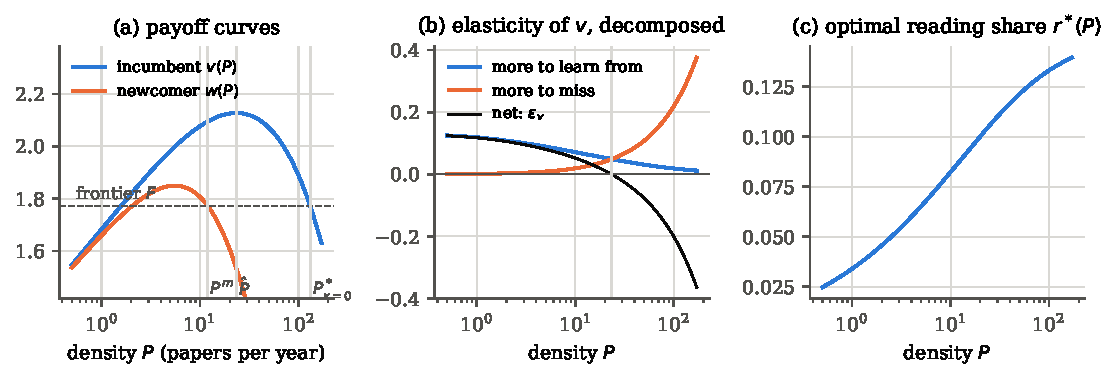
\includegraphics[width=\textwidth]{figures/fig1_payoff_curve.pdf}
\caption{The payoff curve and its two forces. Left: $v(P)$ and the newcomer's
payoff $w(P)=v(P)(1-P/b_c)^\nu$ in the calibrated model, with the peak $\Phat$,
the mature density $P^m$ where $w=F$, and the speed limit $b_c$ at which $w$
vanishes. Right: the decomposition \eqref{eq:envelope} of $v'/v$ into the
learning and overlap terms, and the optimal reading share.}
\label{fig:payoff}
\end{figure}

\paragraph{The value of time.} The envelope theorem also prices every speed-up
inside a topic.

\begin{lemma}[Time shares]\label{lem:timeshares}
At a fixed density, $\partial\ln v/\partial\ln b=r^*(P)/(1-r^*(P))$, while a
faster production speed raises a researcher's payoff by $\dd\ln a$. A speed-up
of a task that takes a share $s_k$ of her time ($s_r=r^*$ for reading,
$s_x=x^*$ for production) by $\dd\ln(\text{speed})$ saves $s_k\,\dd\ln(\text{speed})$
of her time and raises her payoff by $s_k\,\dd\ln(\text{speed})/x^*(P)$. Per unit
of time saved, every speed-up is worth the same, $1/x^*(P)$.
\end{lemma}

The proof is two lines (\cref{app:proofs}). By the envelope theorem
$\partial\ln v/\partial\ln b=r\,\partial_R\ln(QC)\,b$, and the first-order
condition sets $b\,\partial_R\ln(QC)=1/(1-r)$. A 30\% faster reader in a topic
where reading takes 7\% of time therefore gains about two log points, and a
30\% faster producer about 26. The difference is the share of time each task
takes, not anything about entry. It is entry that ranks tools whose value per
hour saved is the same, and \cref{sec:ai} shows how.

\paragraph{The sign of the spillover.} Let one more paper appear in a topic. By
the envelope theorem, the change in every other member's payoff is exactly
$a\,v'(P)$. The researchers' own reallocation of time is second order.

\begin{proposition}[Spillover sign]\label{prop:externality}
An additional paper in a topic of density $P$ changes the per-period payoff of
each incumbent by $a\,v'(P)$. The change is positive for $P<\Phat$ (more to
learn from) and negative for $P>\Phat$ (more to miss).
\end{proposition}

The sign of the spillover is therefore \emph{derived}, not assumed. A paper
helps its topic when the topic is thin and hurts it when the topic is dense.
Overproduction is not built in. Whether science is overcrowded depends on
where equilibrium places topics on $v$. That is the subject of the next two
sections.

\section{Free topic choice without frictions}\label{sec:frictionless}

We first set $b_c=\infty$, so $w=v$. Newcomers move freely between topics and
the frontier. This benchmark isolates the topic-choice margin.

\begin{proposition}[Equilibrium and dissipation]\label{prop:eq}
Let \cref{ass:Q,ass:phi,ass:credit,ass:interior} hold and $b_c=\infty$, and
suppose $\vhat>F(N/n(\Phat),\Phat)$. Then a topic equilibrium exists and is
unique. Every open topic sits on the falling side of the payoff curve,
$P^*>\Phat$, where an additional paper lowers the payoff of every member
(\cref{prop:externality}). Output per researcher equals the frontier value,
$a\,F<a\,\vhat$. The gain from cumulative knowledge, $\vhat-F$, is competed away.
With founders who stay and $\eta_F=0$, the equilibrium density solves
$v(P^*)=e$, whatever the founders' probability $\omega$.
\end{proposition}

Entry continues past the peak because a newcomer compares the \emph{average}
payoff in a topic with the frontier. She ignores that her papers lower everyone
else's payoff once the topic is past $\Phat$. Crossings on the rising side are
unstable: one more entrant raises the payoff of entering. So topics fill past
the peak, to the crossing on the falling side. Founders do not change this.
They earn the same $v(P^*)$ as incumbents, so indifference between founding and
joining pins $v(P^*)$ to what explorers produce.

\begin{remark}[Cities, clubs and topics]\label{rem:henderson}
\Cref{prop:eq,prop:planner} have the structure of the theory of city sizes
\citep{henderson1974} and of clubs \citep{buchanan1965,scotchmer2002}: a single-peaked
average payoff in group size, free entry of new groups, stability only on the
falling side, a planner at the peak of the average payoff, and an entry tax
that decentralises it. Self-organised cities are too large for the same
reason \citep{hendersonbecker2000}. Topics are the cities, newcomers the
migrants, and the frontier the hinterland where new cities are founded. Three
things distinguish topics. The hump is not assumed but derived from the two
jobs of reading (\cref{thm:v}). The congestion is not in land or roads but in
attention: the crowders are the readers, so whether an extra member helps or
hurts is decided by where the topic sits on its payoff curve
(\cref{prop:externality}). And the object the data measure, the duplication rate,
is a function of density alone, which makes the invariance of
\cref{prop:volume} a testable restriction rather than a curiosity.
\end{remark}

\paragraph{Volume opens new topics.} The next result says how a larger
community distributes itself.

\begin{proposition}[Volume opens new topics]\label{prop:volume}
In the large-topic limit, equilibrium density depends on $(N,a)$ only through
the product $N a$, and
\begin{equation}\label{eq:E}
\mathcal E\equiv\frac{\dd\ln P^*}{\dd\ln N}=\frac{\eta_F}{\eta_F\,D+|\eps_w|+\theta_F\,\eps_U},\qquad D\equiv1-\eps_x+\frac{\rho}{\delta}\,\frac{P^*/b_c}{1-P^*/b_c}\ge 1,
\end{equation}
where $\eps_w=\dd\ln w/\dd\ln P<0$, $\eps_x=\dd\ln x^*/\dd\ln P\le 0$ and
$\eps_U=\dd\ln\bar U_F/\dd\ln P$ are evaluated at $P^*$ ($\eps_U=\eps_v$ in the
stationary economy). New topics absorb a share $\dd\ln M^*/\dd\ln N=1-D\,\mathcal E$
of growth, and papers per researcher move with elasticity $\eps_x\mathcal E\le 0$.
If the frontier is not depleted ($\eta_F=0$), density, the overlap rate and the
aware share do not depend on $N$, $a$ or the cost of entering science.
\end{proposition}

\Cref{eq:E} holds for any $b_c$, and we use it again in
\cref{sec:catchup,sec:ai}. Three remarks.

First, the overlap rate is \emph{pinned by entry, not by volume}. When the
community grows, newcomers open new topics until existing ones are no more
attractive than the frontier. The flagged overlap rate and the aware share are
functions of $P^*$ alone (\cref{lem:credit}), so they inherit its invariance. A
flat overlap rate while submissions double (Fact~\ref{fact:volume}) is what the
model predicts. It is not evidence that crowding is harmless.

Second, a fixed field corresponds to $\eta_F\to\infty$. Then $\mathcal E\to1/D$:
growth thickens existing topics. The arXiv elasticities of 0.12--0.19 at broad
radii and 0.035 (SE 0.118) at the closest-overlap radius, against fixed-field
benchmarks of 0.53--0.81 (Fact~\ref{fact:volume}), imply that most growth opens
new ground. Inverting \eqref{eq:E},
\begin{equation}\label{eq:eta}
\eta_F=\frac{\mathcal E\,\big(|\eps_w|+\theta_F\eps_U\big)}{1-\mathcal E\,D},
\end{equation}
so the frontier's depletion is identified by the volume elasticity, the slope
of the newcomer's payoff curve and the founders' share. The inversion assumes
that the frontier did not move for other reasons over the sample. A frontier
that improved, for instance because founding got easier, would lower measured
density growth and bias $\eta_F$ down (\cref{thm:incidence}).

Third, papers per author barely move when the community grows, because
$\eps_x\mathcal E$ is the product of two small numbers. Faster production, by
contrast, raises papers per author one for one (\cref{prop:ai}). The two can
be told apart only at the author level, because entrants change the
composition of authors (Fact~\ref{fact:authors}).

\begin{remark}[Short-run and long-run elasticities]\label{rem:shortrun}
\Cref{prop:volume} compares steady states, while the arXiv elasticities are
measured over 2018--2025, a period in which volume grew about 12\% a year. In
the model, mature topics adjust to a change in $N$ at once, since the marginal
newcomer is indifferent. The only wedge between the measured and the
steady-state elasticity is composition. Faster growth means more young topics,
which are thinner. If an area's growth rate rises by $\dd g$ for $T$ years,
its age weights for topics younger than $T$ scale by $e^{\dd g(T-a)}$ and its
log volume rises by $T\dd g$, so
\begin{equation}\label{eq:shortrun}
\mathcal E_{\text{measured}}=\mathcal E+\frac{\operatorname{Cov}_\omega\big(\ln P,(T-a)^+\big)}{T}+o(\dd g),
\end{equation}
where $\operatorname{Cov}_\omega$ is the researcher-weighted covariance over the
cross-section of topic ages $a$. The covariance is negative because young topics
are thin, so the measured elasticity is a lower bound. In the calibrated
life cycle the bias over a seven-year window is $-\calCompBias$
(\cref{sec:quant}). The long-run elasticity is therefore at most about
$\calCompBias$ above the measured one, which leaves the conclusion that
volume mostly opens new ground intact. Steady growth at a constant rate does
not bias the estimate at all, because area fixed effects absorb a constant age
composition.
\end{remark}

\begin{remark}[Reading capacity per researcher or per field]
Consider instead a fixed screening capacity $B$ per field, so that coverage is
$B/P$ and researchers produce full time. Topic choice still pins density, so
\cref{prop:eq,prop:volume} survive. But if topics cannot split, overlap rises
with field volume, which the arXiv volume test rejects. Per-researcher
capacity also keeps the time-allocation margin that prices tools by the time
they save (\cref{lem:timeshares}). We adopt it throughout.
\end{remark}

\begin{figure}[t]
\centering
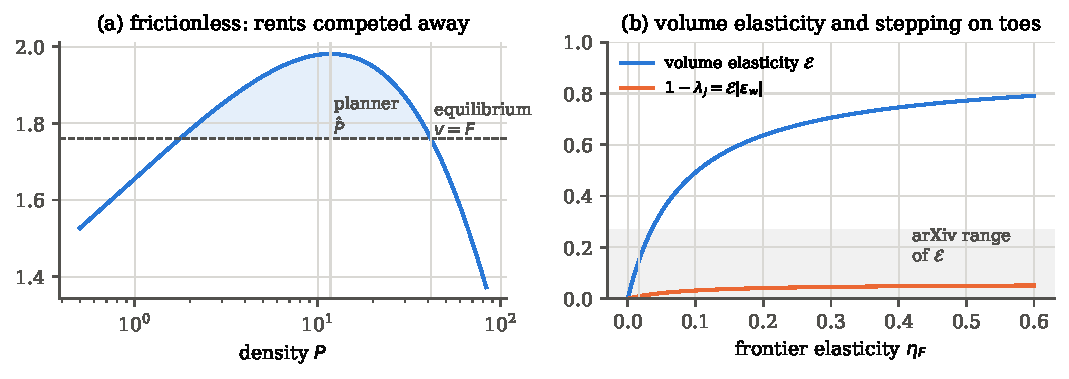
\includegraphics[width=\textwidth]{figures/fig2_planner_volume.pdf}
\caption{Left: without catch-up costs, topics fill to the density where $v=F$,
and the shaded rent between the payoff curve and the frontier is competed away;
the planner puts topics at the peak. Right: the volume elasticity
$\mathcal E$ and the stepping-on-toes wedge $\mathcal E|\eps_w|$ as functions of
the frontier's depletion $\eta_F$, at the calibrated slope of $w$ and founders'
share. The shaded band is the range of arXiv estimates of $\mathcal E$.}
\label{fig:planner}
\end{figure}

\paragraph{The planner.} A planner who controls how many researchers join each
topic, but not how they split their time, maximises output subject to births
equalling deaths and researchers adding up.

\begin{proposition}[Overcrowding and the frontier subsidy]\label{prop:planner}
Let the conditions of \cref{prop:eq} hold, with $b_c\le\infty$ and $\eta_F=0$.
\begin{enumerate}[label=(\roman*)]
\item In the large-topic limit output per researcher at any common density is $a\,w(P)$, so the planner puts every topic at the peak of the newcomer's payoff curve, $P^o=\hat P_w$, which is the peak of $v$ when $b_c=\infty$. She opens more topics and puts fewer researchers in each. The gain in output per researcher is $\hat w/F-1$.
\item With explorers counted and founders who do not stay ($\omega=0$), the planner's density satisfies
\begin{equation}\label{eq:plannerfoc}
\frac{w(P^o)-e}{w(P^o)}=|\eps_w(P^o)|\,\frac{1+s\,n(P^o)/\xi}{D(P^o)},
\end{equation}
with $\hat P_w<P^o<P^*$. Overlap stays positive at the optimum.
\item In the stationary economy a frontier subsidy (equivalently, a tax on joining open topics) of $s^o=\hat w-F(M^o,\hat P_w)$ per unit of production speed decentralises the large-topic optimum.
\item (Two wedges) A planner who also chooses $x$ wants researchers to produce less than $x^*(P)$ wherever $w'(P)<0$ and more wherever $w'(P)>0$. The production wedge is proportional to $(\ln w)'(P)$. In the large-topic limit it vanishes at the optimal density, so controlling topic choice alone attains the first best.
\end{enumerate}
\end{proposition}

There are two wedges, and they differ in importance. Newcomers choose topics
on the average payoff while the planner uses the marginal one: this is the
\emph{crowding wedge}. Inside each topic, researchers ignore that their papers
add to what colleagues must read: this is the \emph{production wedge}. Part
(iv) shows the production wedge is a symptom of the crowding wedge. Once topics
are at their best density, researchers' private time allocation is efficient.
Part (iii) holds in the stationary economy. In an economy where topics are born
thin and grow, a flat subsidy to the frontier also deters the first followers
of newborn topics, and the policy has to depend on a topic's age
(\cref{prop:policy}). The welfare criterion here is total private credit;
\cref{prop:social} shows that the overcrowding result survives when part of
that credit is a transfer, and \cref{prop:audience} values output by
readership instead.

\section{Catch-up, the speed limit and rents}\label{sec:catchup}

The frictionless benchmark predicts equal returns across topics. The arXiv data
reject this (Fact~\ref{fact:hump}). The same researcher earns more citations in
denser topics over most of the density range, and less in the densest ones. We
now let $b_c<\infty$: newcomers must read a topic's stock before contributing,
while its literature keeps growing.

\subsection{Mature topics}

\begin{proposition}[Mature topics under catch-up costs]\label{prop:mature}
Let \cref{ass:Q,ass:phi,ass:credit,ass:interior} hold and $b_c<\infty$.
\begin{enumerate}[label=(\roman*)]
\item $w(P)=v(P)(1-P/b_c)^\nu$ is strictly log-concave on $(0,b_c)$, with a unique peak $\hat P_w<\min\{\Phat,b_c\}$, and vanishes at $b_c$.
\item In a topic equilibrium the mature density $P^m$ solves $w(P^m)=F$ on the falling side of $w$, and $P^m<b_c$. Incumbents earn $a\,v(P^m)$ per period. Their log premium over the frontier equals the catch-up cost, $\ln[v(P^m)/F]=-\nu\ln(1-P^m/b_c)=(\rho+\xi)\,T(P^m)$.
\item Mature topics lie on the \emph{rising} side of $v$ if and only if catch-up is costly relative to the rent at the peak: $\Phat\ge b_c$, or $\nu\ln(1-\Phat/b_c)<\ln(F/\vhat)$.
\item Let topics differ in fertility $\zeta$, so that payoffs are $\zeta v(P)$, and let $P^m(\zeta)$ solve $\zeta w(P)=F$. Across mature topics, log returns rise with log density with slope equal to the catch-up elasticity,
\[
\frac{\dd\ln[\zeta\,v(P^m(\zeta))]}{\dd\ln P^m(\zeta)}=\eps_\Gamma(P^m)\equiv\nu\,\frac{P^m/b_c}{1-P^m/b_c},
\]
which exceeds the premium $-\nu\ln(1-P^m/b_c)$.
\end{enumerate}
\end{proposition}

Catch-up turns the dissipated rent into a protected one. Incumbents earn more
than the frontier, and the premium exactly offsets what a newcomer gives up
while she reads her way in. More fertile topics attract more entrants, have
larger stocks and so protect larger premia. This yields a positive
returns--density gradient across topics, whether those topics lie left or
right of $\Phat$. In the data the same gradient also reflects audience size,
since a paper with more close neighbours has more potential citers. The
measured gradient of 6.7\% per standard deviation (Fact~\ref{fact:hump}) is
therefore an upper bound on the catch-up channel. We use it as such in
\cref{sec:quant}.

\subsection{The speed limit}

\begin{theorem}[Speed limit]\label{thm:speed}
Let $b_c<\infty$.
\begin{enumerate}[label=(\roman*)]
\item \emph{(Closure.)} A topic whose flow is at least $b_c$ is closed to newcomers: anyone who joins it while its flow stays there never catches up. Its incumbents' rents are protected however large they are.
\item \emph{(Rents near the limit.)} Every mature topic satisfies $P^m<b_c$. As fertility rises, $P^m(\zeta)\to b_c$, and both the incumbents' premium and the cross-topic returns gradient diverge; the gradient grows faster than the premium.
\item \emph{(Growing topics.)} Myopic entry into a topic that grows stops before its flow reaches $b_c$, however fast it grows.
\item \emph{(Production shocks close topics.)} A production speed-up by the factor $1+\alpha$ raises the flow of every topic on impact, before membership adjusts, by the same factor at given reading shares. Every topic with $P^m>b_c/(1+\alpha)$ closes, and stays closed for at least $\ln[(1+\alpha)P^m/b_c]/\rho$ periods while turnover thins it.
\end{enumerate}
\end{theorem}

The theorem makes ``too fast'' precise. A literature can grow faster than the
people outside it can absorb, and when it does, the topic is shut to
newcomers however rewarding it is for those inside. Near the limit, small
differences in fertility produce large differences in returns, so the speed
limit is also where the returns gradient is steepest. Part (iv) is the version
that matters for artificial intelligence. A tool that lets everyone produce
faster raises every topic's flow at once, and the topics that were already
densest are pushed past the limit until turnover brings them back. Entry, and
the turnover of people and ideas that comes with it, stops there for a while.
This is one mechanism behind the slowed progress of large fields documented by
\citet{chuevans2021}: when papers arrive faster than newcomers can absorb them,
attention stays with the established canon. Better catch-up tools, such as
reviews and summaries, raise the limit.

\subsection{Rising incumbent returns, falling newcomer returns}

The interesting object is the gap between what incumbents earn, $v$, and what a
newcomer can expect over her spell, $w=v\Gamma$. Incumbents never pay the
catch-up cost again. Newcomers and the planner do. The welfare statement
follows almost by definition of stability, so we state it as a corollary and
put the weight on what it implies for measurement.

\begin{corollary}[Overcrowding with rising returns]\label{cor:overcrowd}
In every stable topic equilibrium, one more member in a topic of density $P$
changes total output of the other members by $n\,a\,w'(P)\,\dd P/\dd n<0$.
This counts both the spillover on incumbents ($v'$) and the extra catch-up she
imposes on future newcomers ($v\,\Gamma'$). If $w(\Phat)<F$, then
$\hat P_w<P^m<\Phat$: incumbents' returns rise with density ($v'(P^m)>0$) while
the topic is too crowded ($w'(P^m)<0$). The loss of output per researcher in
the large-topic limit is $1-F/\hat w$.
\end{corollary}

The measured gradient is the incumbents' private return to density. A
newcomer values a topic net of the reading she must do to join it, and so does
the planner. Rising incumbent returns are the footprint of the catch-up rent,
not of an untapped spillover. A natural reading of Fact~\ref{fact:hump} is that
most researcher-years sit where more density raises returns, so most topics are
too thin. The corollary says that this reading conflates $v$ with $w$. Two
kinds of topic can be too thin. The first is young topics that have not yet
filled. The second, if the frontier is attractive enough, is newborn topics that
never find followers (\cref{rem:coordination}).

\begin{remark}[Newborn topics]\label{rem:coordination}
A newborn topic has no stock, so its first follower needs no catch-up and
earns $v(P_0)$, where $P_0$ is the flow of a newborn topic. Newborn topics
attract followers if and only if $v(P_0)>F$. (The condition is on $v$, not on
$w$: a stationary topic of density $P_0$ would carry a stock, a newborn one
does not.) If $F>v(P_0)$, newborn topics attract no followers, although a
coordinated group would earn $\vhat>F$. Science then holds too many topics that
are too small, and the planner would fix it by seeding followers. When
$v(P_0)>F>w(P_0)$, as in the calibration, a newborn topic is worth joining
while its stock is empty, but a stationary topic of the same density is not.
The topic must grow fast enough for its stock to lag behind its flow, or
entry stalls before the topic is worth joining in its own right
(\cref{prop:toofast}). Policies that raise the frontier value by more than
$v(P_0)-F$ shut down the birth of new topics (\cref{prop:policy}).
\end{remark}

\subsection{Social value and priority transfers}

The welfare statements so far count private credit. Priority credit is partly a
transfer \citep{merton1957,hillstein2025}. When a later paper turns out to
duplicate an earlier one, some of the credit it loses goes to the earlier
paper, so part of the ``loss'' from overlap is redistribution. Conversely, a
duplicate may be worth less to science than its residual citations suggest. We
therefore separate social value from credit. Let the social value of a project
be $Q\,C_s$, with
\[
C_s(R,P)=\exp\{-\theta P[\lambda_s-\Delta_s\varphi(R/P)]-\theta_c\lambda_cP\},
\]
where $\lambda_s$ is the share of a project's social value lost per unread
covering paper and $\Delta_s$ the part of it that detection averts. Researchers
still choose $r^*(P)$ to maximise credit, and social output per unit of
production speed in a topic of density $P$ is
$s(P)=(1-r^*)\,Q(br^*,P)\,C_s(br^*,P)$, with $s_w(P)=s(P)\Gamma(P)$. The
catch-up cost is a real resource cost, reading time, and is not a transfer.

\begin{proposition}[Social value]\label{prop:social}
\begin{enumerate}[label=(\roman*)]
\item One more member changes the social output of the others by $n\,a\,s_w'(P)\,\dd P/\dd n$, where
\[
\frac{s'(P)}{s(P)}=\frac{v'(P)}{v(P)}-\theta\big[(\lambda_s-\lambda)-(\Delta_s-\Delta)\psi(c^*)\big]+\theta b(\Delta_s-\Delta)\varphi'(c^*)\,r^{*\prime}(P),
\]
with $\psi(c)=\varphi(c)-c\varphi'(c)\ge0$.
\item \emph{(Uniform wedge.)} If $\Delta_s=\Delta$, then $s(P)=v(P)e^{-\theta(\lambda_s-\lambda)P}$ exactly. Social and private values then differ by a factor that rises or falls exponentially in density. The equilibrium is overcrowded relative to the social optimum if and only if the share of overlap losses that are transfers, $\tau\equiv(\lambda-\lambda_s)/\lambda$, satisfies
\[
\tau<\frac{|\eps_w(P^m)|}{\theta\lambda P^m}.
\]
In particular overcrowding is stronger when duplicates are worth less to science than to their authors ($\lambda_s>\lambda$).
\item \emph{(Proportional transfer.)} If a share $\tau$ of every overlap loss is a transfer, $\ln C_s=(1-\tau)\ln C$, the social optimum density maximises $\ln v(P)-\tau\ln C^*(P)+\ln\Gamma(P)$, where $C^*(P)=C(br^*(P),P)$.
\end{enumerate}
\end{proposition}

Part (ii) gives a sharp test. Overcrowding survives any degree of transfer as
long as the slope of the newcomer's payoff curve at the mature density exceeds
the expected erosion intensity $\theta\lambda P^m$. In the calibrated model the
slope is \calEpsW\ against an erosion intensity of \calThetaLamPm, so the
critical transfer share is \calTauCrit, above one. Under proportional
transfers (part (iii)), the social optimum moves from \calPsocialZero\ to
\calPsocialFull\ papers a year if all overlap losses are transfers, still below
the mature density of \calPm. Transfers therefore shrink the welfare gain from
optimal topic choice, from \calPlannerGain\ to \calGainTransfer\ of output per
researcher, but they do not reverse its sign. The catch-up burden that newcomers
impose on one another is a real resource cost, and on its own it keeps mature
topics too dense. The transfer critique matters for magnitudes, and especially
for the frictionless benchmark, where the dissipated rent is a difference in
private payoffs; it does not matter for the direction of the inefficiency.

\section{Artificial intelligence as several different shocks}\label{sec:ai}

``AI'' enters the model through several parameters, and each leaves a different
footprint. That is what makes the model testable rather than a story.

\begin{proposition}[Signatures of AI]\label{prop:ai}
In the large-topic limit:
\begin{enumerate}[label=(\roman*)]
\item \emph{Faster drafting} ($a\uparrow$) acts like a larger community. Density moves with elasticity $\mathcal E$ (zero if $\eta=0$) and the number of topics with elasticity $1-D\mathcal E$. Papers per researcher rise with elasticity $1+\eps_x\mathcal E$, and output per researcher with elasticity $1-\mathcal E|\eps_w|$.
\item \emph{Cheaper entry into science} ($c\downarrow$, with $N$ set by $aF(M)=\omega+c$ and $\eta>0$) raises $N$. Density rises with elasticity $\mathcal E$ with respect to $N$, papers per researcher move with elasticity $\eps_x\mathcal E\approx 0$, and new topics absorb a share $1-D\mathcal E$ of growth.
\item \emph{Better reading, learning or search, or cheaper pivots} ($b$, $\beta$ or $\sigma\uparrow$, $\kappa_p\downarrow$) raise $v$ and $w$ at every density. Density rises and the number of topics falls: science concentrates. Output per researcher rises only through the frontier, by $\eta\,|\dd\ln M^*|$, and is unchanged when $\eta=0$.
\item \emph{Faster catch-up} ($b_c\uparrow$, e.g.\ literature-summarising tools) raises $w$ at every density, with the effects in (iii). It also lowers the overshooting threshold $g^*$ of \cref{prop:toofast}, so more topics grow too fast.
\item \emph{Better search} ($\sigma\uparrow$) raises the aware share $A$ at any given reading coverage.
\end{enumerate}
\end{proposition}

Parts (iii) and (iv) follow from the envelope theorem. Each parameter raises
$g(r,P)$ at every $(r,P)$, hence raises $v$. A pointwise upward shift of a
single-peaked curve moves its falling-side crossing with a fixed $F$ to the right.
The effect on the measured overlap rate is ambiguous in general: denser topics
generate more overlap, but better detection removes more of it.
\Cref{tab:ai} reports the calibrated signs.

\begin{table}[t]
\centering
\caption{The footprints of AI in the calibrated model}\label{tab:ai}
\small
\begin{tabular}{@{}llrrrrrrr@{}}
\toprule
Channel & Shock & Density & Topics & Papers/ & Output/ & Flagged & Aware & $g^*$ \\
 & & & & researcher & researcher & overlap & share (pp) & (pp) \\
\midrule
Faster drafting & $a\times1.3$ & +5.1 & +20.0 & +26.1 & +25.4 & +6.7 & -1.3 & +0.0 \\
Cheaper entry & $N\times1.3$ & +5.1 & +20.0 & -0.1 & -0.8 & +6.7 & -1.3 & +0.0 \\
Faster reading & $b\times1.3$ & +8.5 & -9.9 & +0.2 & +0.4 & +1.6 & +5.8 & +0.5 \\
Better learning & $\beta\times1.3$ & +13.6 & -16.9 & -0.5 & +0.7 & +17.0 & -2.7 & -5.6 \\
Better search & $\sigma\times1.3$ & +0.3 & -0.4 & +0.0 & +0.0 & -12.4 & +11.1 & +0.6 \\
Faster catch-up & $b_c\times 2$ & +61.3 & -61.3 & -1.5 & +2.6 & +79.5 & -13.6 & -23.6 \\
Cheaper pivots & $\kappa_p\div 2$ & +1.1 & -1.4 & -0.1 & +0.1 & -21.6 & -15.3 & +0.6 \\
\bottomrule
\end{tabular}
\par\smallskip\footnotesize Long-run stationary effects in log points ($\times100$) of a 30\% shock (catch-up speed doubled, pivot cost halved). Density is $P^*$; output per researcher is $aF(M^*)$. The flagged overlap rate is relative to its baseline level, which is a normalisation (\cref{sec:facts}). $g^*$ is the overshooting threshold of \cref{prop:toofast}.

\end{table}

\paragraph{What the arXiv data say.} The footprints differ enough to tell the
channels apart. Four facts settle the question for 2023--2026.
\begin{itemize}
\item Papers per author stayed flat while authors grew (Fact~\ref{fact:authors}). Faster
drafting raises papers per author one for one. Cheaper entry leaves them flat.
\item High-uptake areas produced \emph{more} pioneer papers and \emph{lower} local
density relative to their own pre-ChatGPT trend (Fact~\ref{fact:concentration}). All reading-side channels predict
concentration: fewer new topics and denser old ones. Cheaper entry predicts more
new topics. Faster growth also raises the share of young, thin topics in the
life-cycle model, which lowers mean density.
\item The aware share of close overlap stayed at 35--42\% (Fact~\ref{fact:aware}). Better search
would have raised it.
\item Measured by meaning, close overlap did not fall (Fact~\ref{fact:wording}). Under cheaper entry it is
nearly pinned, because $\mathcal E$ is small (\cref{prop:volume}).
\end{itemize}
So far AI has acted on science through \emph{entry}. The reading channels remain
predictions. When literature-summarising tools spread, the model predicts
denser topics, fewer new ones, more overshooting by fast-growing topics, and
little or no gain in output per researcher.

\paragraph{Writing AI scales science; reading AI crowds it.} The asymmetry in
\cref{prop:ai} is the paper's sharpest policy implication. Writing speed
multiplies every payoff, including the frontier's. Newcomers spread out, so a
faster pen raises output almost one for one and leaves duplication nearly
unchanged in the long run.
Reading speed improves only existing topics. Newcomers crowd in until those
topics are no better than the frontier, so the improvement is competed away.
This overturns a natural intuition. The worry that writing tools will flood science
with duplicates is misplaced in the long run: free topic choice pins overlap.
The costs of a faster pen are transitional (\cref{app:extensions}) and
concentrated in topics that grow too fast. The hope that
reading tools will raise productivity is also misplaced: free topic choice
dissipates their gains. Tools are worth subsidising only if they make new topics easier
to open, that is, if they raise $F$.

\section{Seven facts from arXiv}\label{sec:facts}

The evidence comes from the project's pre-registered tests on 1.71 million
arXiv papers posted 2018--2025, classified into 150 text-based fine areas.
These are complemented by a PDF sample of 25,400 papers for citation behaviour and OpenAlex
citation counts. A paper's \emph{overlap flag} is set when an earlier paper by
another group, posted 3 to 24 months before, lies above its area's 99th
percentile of 2018--19 nearest-neighbour similarity. The \emph{level} of the
flagged rate is therefore a normalisation, about 1\% in the base period. Its
\emph{changes} carry the information. Every prediction tested below was written
down before the test was run. \Cref{tab:facts} collects the numbers.

\begin{enumerate}[label=\textbf{Fact \arabic*.},ref=\arabic*,leftmargin=*]
\item\label{fact:volume} \emph{Volume opens new ground.} The elasticity of the
local-neighbour hazard with respect to an area's prior two-year volume is
0.04--0.19 across similarity radii, with area and year effects. If an area's
papers kept landing in the same idea space, randomly thinning each paper's
observed neighbour list implies 0.53--0.89. In the all-arXiv time series, volume
rose 113\% from 2018 to 2025 while the overlap hazard rose 13\% (elasticity
0.19--0.27). Close overlap responds least of all.

\item\label{fact:authors} \emph{Growth came from new authors.} Papers per author
stayed flat while the number of authors grew.

\item\label{fact:hump} \emph{Returns are hump-shaped in topic density.} Comparing
the same researcher across years spent in denser or sparser topics, with author
and year effects (923,000 author-years), one standard deviation of density goes
with 6.7\% more fractional citations per author-year. By fifth of density,
returns relative to the middle fifth are $-8\%$ in the sparsest fifth, rise to
$+5\%$, and fall back to $+1\%$ in the densest. A quadratic puts the peak about
one standard deviation above mean density, with 12\% of researcher-years beyond
it. The shape survives using the third-closest paper and restricting to
researchers active three or more years.

\item\label{fact:credit} \emph{Duplicates lose some credit, aware follow-ons gain.}
Relative to papers in the same area-year with the same topic density,
\emph{unaware} overlaps (which do not cite their nearest earlier paper) receive
19\% fewer citations. \emph{Aware} overlaps (which cite it) receive 29\% more.

\item\label{fact:aware} \emph{Awareness did not rise.} The aware share of close
overlap stayed between 35\% and 42\% in every year from 2019 to 2026. It did not
differ by exposure to large language models: $-0.5$ pp per standard deviation,
SE 1.4.

\item\label{fact:concentration} \emph{No concentration where LLMs spread.}
High-uptake areas were already losing pioneer papers before ChatGPT. Against
their own extended trend, they produced \emph{more} pioneer papers afterwards:
$+0.4$ pp (SE 0.3) in 2023--2025H1 and $+1.3$ pp (SE 0.5) from 2025H2. Local density
fell by 1.1 and 2.7 pp.

\item\label{fact:wording} \emph{The 2026 drop in measured overlap is a change in wording.}
Word-based (TF-IDF) overlap fell in 2026 across the whole similarity
distribution, concentrated in high-uptake areas rather than dense ones. Measured
by meaning (sentence embeddings), close overlap did not fall.
\end{enumerate}

\begin{table}[t]
\centering
\small
\caption{Targets and tests from the arXiv evidence}\label{tab:facts}
\begin{tabularx}{\textwidth}{@{}lXl@{}}
\toprule
Fact & Statistic & Value \\
\midrule
1 & Elasticity of local density to area volume & 0.04--0.19 (time series 0.19--0.27) \\
  & Fixed-field benchmark & 0.53--0.89 \\
2 & Papers per author while authors grew & flat \\
3 & Citations per author-year per SD of density (author FE) & $+6.7\%$ (SE 0.15) \\
  & By fifth, relative to middle: sparsest / 4th / densest & $-8\%$ / $+5\%$ / $+1\%$ \\
  & Peak of quadratic; share of researcher-years beyond it & $\approx+1$ SD; 12\% \\
4 & Citations: unaware overlap / aware overlap & $-19\%$ (2) / $+29\%$ (5) \\
5 & Aware share of close overlap, 2019--2026 & 35--42\%, flat \\
6 & Pioneer papers vs.\ trend, high-uptake areas, 2025H2+ & $+1.3$ pp (0.5) \\
7 & Close overlap by meaning, high- vs.\ low-uptake, 2024--26H1 & $-0.19$ pp (0.24) \\
\bottomrule
\end{tabularx}
\begin{minipage}{\textwidth}\footnotesize\smallskip
Notes: arXiv 2018--2025, 150 areas. Standard errors in parentheses. Facts 1 and
3 discipline the calibration of \cref{sec:quant}. Facts 2 and 5--7 test the AI
channels of \cref{sec:ai}. Fact 4 disciplines the credit block.
\end{minipage}
\end{table}

How do the facts map into the model? Fact~\ref{fact:volume} is the volume
elasticity $\mathcal E$ of \cref{prop:volume}. Fact~\ref{fact:hump} rejects the
equal returns of the frictionless model and motivates the catch-up cost of
\cref{sec:catchup}. Fact~\ref{fact:credit} disciplines the credit parameters $\lambda$ and
$\Delta/\lambda$ (\cref{lem:credit}). Facts~\ref{fact:authors} and
\ref{fact:aware}--\ref{fact:wording} distinguish the AI channels of \cref{sec:ai}.

\section{Evidence II: arXiv's rules as experiments}\label{sec:causal}

The facts above are correlations. This section uses arXiv's own rules, which
create variation in how much a paper is read, in the cost of entering, in the
cost of catching up on a literature and in how much one person may write. The
data are the arXiv metadata snapshot of 18 October 2026 \citep{kaggle2026}:
2.2 million papers with new-style identifiers submitted from 2015 to 15
October 2026, with the exact time of each submission, the submitter's name,
the author list and the abstract. \Cref{app:data} documents every construction.
\Cref{tab:listing,tab:policies} report the estimates.

\paragraph{Reconstructing the daily listings.} arXiv announces new papers once a
day. Papers submitted before the daily cutoff appear in that evening's listing,
and later papers wait for the next one. Identifiers are assigned at announcement,
in listing order. Within an announcement batch, the rank correlation between
identifier and submission time is 0.98 for papers that were not held for
moderation (median across batches). Six percent of papers are held and announced
later. The submission-time distribution reveals the cutoff. It was 16:00
Eastern Time until the end of 2016 and has been 14:00 since January 2017. On an
average weekday about 15 papers are submitted in the first ten seconds after 14:00:00:
authors race for the top of the next listing \citep{haqueginsparg2009}. We
place every paper in its announcement batch and rank it within its primary
category's list of new submissions.

\subsection{Does reading protect? Listing position as a readership shock}

\Cref{lem:credit} gives sharp predictions for a shock that makes a paper $i$
more visible to the researchers who might later cover it. If visibility raises
the probability $\varphi$ that a later covering project detects $i$, unaware
duplicates of $i$ fall by $\theta\,\dd\varphi$, aware follow-ons that cite $i$
rise by $q\theta\,\dd\varphi$, and the ratio of the two effects identifies $q$,
the share of detections that proceed. We test these predictions with two
designs.

\paragraph{Design A: the daily cutoff.} A paper submitted just after 14:00 opens
the next listing, while one submitted just before closes the current one. The
first stage is sharp (\cref{tab:listing}, panel A; \cref{fig:listing}). Within an
hour of the cutoff, excluding a five-minute donut around the bunching, crossing
the cutoff raises the probability of being among the first five papers by
\empRDtopfive, from a base of \empRDtopfiveBefore. The comparison it delivers,
however, is first against \emph{last}. The end of a listing is also highly
visible, a ``reverse visibility'' effect documented for arXiv by
\citet{haqueginsparg2010} and for NBER working papers by
\citet{feenbergetal2017}. Submitters on the two sides also differ: those just
after the cutoff have fewer prior submissions (\empRDprior, SE \empRDpriorSE). Top-of-listing papers receive \emph{fewer} citations
than end-of-listing papers: \empRDcitesIns\ log points (SE \empRDcitesInsSE) in
high-energy physics, where INSPIRE-HEP gives complete citation counts, and
\empRDcitesSS\ (SE \empRDcitesSSSE) across all fields in the
\empRDcitesSSN\ papers with Semantic Scholar counts. The cutoff therefore does not isolate
visibility, and we do not use it to test detection.

\paragraph{Design B: rank within the listing.} A cleaner source of variation is
how many other papers happen to be submitted earlier on the same day. A
paper's position is one plus the number of papers in its category submitted
since the batch opened. We hold fixed the submission time (in 15-minute bins,
separately for the weekend batch), the category-year, the announcement date
and the size of the listing. Position then varies only with the timing of
other people's submissions. We use all \empRankN\ papers in the nine
categories covered by INSPIRE-HEP in 2017--2022, excluding the first 15 minutes
after the cutoff. The residual standard deviation of log position is
\empRankSD. Predetermined characteristics are balanced: number of authors and
the submitter's prior submissions are unrelated to residual position.
Abstracts are slightly shorter lower in the list (1.6 words of 151 per log point, SE 0.6).

The readership effect is small. One log point lower in the listing, roughly
moving from second to fifth place, reduces citations by \empRankCites\ log points
(SE \empRankCitesSE; \empRankCitesMain\ without date fixed effects). Position bins show
no premium for the very first slots once dates are held fixed. Later overlapping
work responds even less. We count later papers in the same category, within 24
months, by authors who do not overlap with the focal paper's, whose TF-IDF
similarity exceeds the category's median (75th percentile) of nearest-neighbour
similarity. With INSPIRE's curated reference lists we split them into those
that cite the focal paper (aware) and those that do not (unaware). One log point
lower in the listing changes unaware overlap at the 75th percentile threshold by
\empRankUsevfive\ (SE \empRankUsevfiveSE) on a mean of \empRankUsevfiveMean, and
aware overlap by \empRankAsevfive\ (SE \empRankAsevfiveSE). The 95\% interval
rules out an increase in unaware overlap of more than \empRankUsevfiveUB\ per log
point. The minimum detectable effect at 80\% power is \empRankUsevfiveMDE\ of the
mean. Self-follow-ups by the focal paper's own authors fall with position
(\empRankSelf, SE \empRankSelfSE). This suggests that attention encourages authors
to continue a line of work, or that the design leaves some day-level confounding;
either way it does not affect the comparison with other authors' work.

\paragraph{What this teaches.} Passive visibility moves casual readership a little
and does not move the detection of overlapping work. In the model, detection
depends on the coverage $R/P$ that a later researcher chooses and on search
precision $\sigma$, not on how prominently the earlier paper was announced. The
result says that the protective job of reading is done by targeted search when a
project is planned or written up, not by browsing daily listings. This matches
the high calibrated search precision needed for a 60\% aware share
(Fact~\ref{fact:aware}). The right causal test of $\varphi$ is therefore a
shock to the cost of search. \Cref{sec:predictions} sets out one: the blocking
of Google in mainland China from 2014 \citep{zhengwang2020}. The model predicts
that it lowered the aware share and raised unaware duplication in work by
China-based authors, relative to Hong Kong-based and overseas Chinese authors
in the same topics.

\begin{figure}[t]
\centering
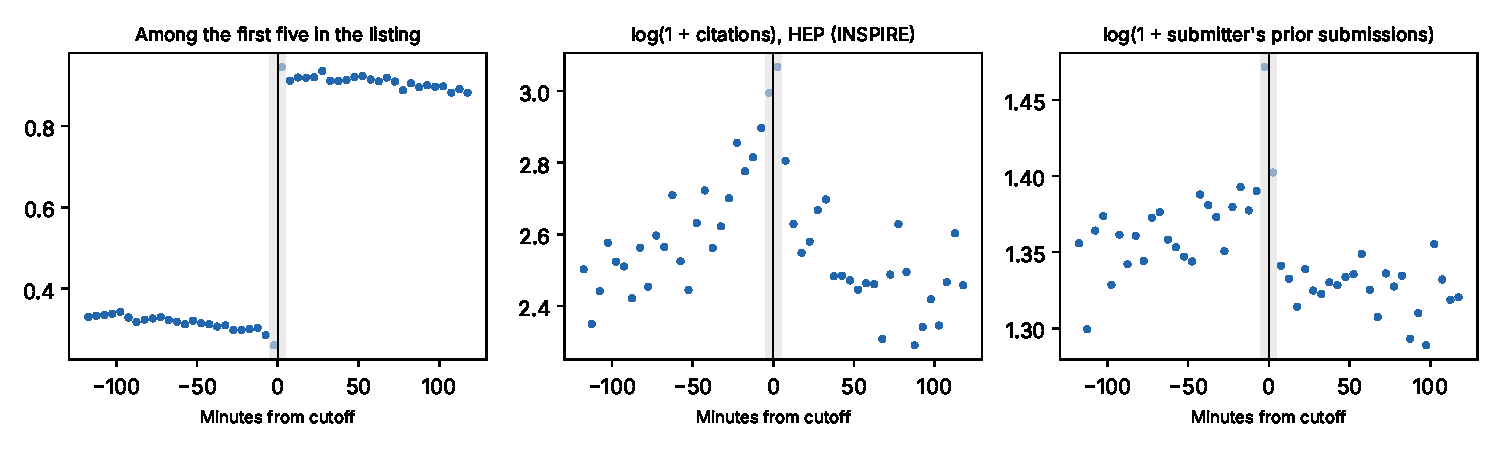
\includegraphics[width=\textwidth]{figures/emp_rd_listing.pdf}
\caption{The daily cutoff. Binned means, net of category-year means, by minutes
from the 14:00 ET cutoff (weekday submissions 2017--2022; shaded: five-minute
donut). Left: probability of being among the first five papers of the
category's listing. Middle: log citations in high-energy physics (INSPIRE-HEP).
Right: the submitter's prior submissions, a predetermined characteristic that
jumps at the cutoff. Papers just after the cutoff open the next listing; papers
just before close the current one.}
\label{fig:listing}
\end{figure}

\begin{table}[p]
\centering\footnotesize
\caption{Listing position, readership and later overlapping work}\label{tab:listing}
\begin{tabular}{@{}lrrrl@{}}
\toprule
Outcome & Estimate & (SE) & Mean & $N$ \\
\midrule
\multicolumn{5}{@{}l}{\emph{A. Discontinuity at the daily cutoff: submitted just after (top of next listing) vs.\ just before (end of current listing)}} \\
Position in listing (0 = top, 1 = bottom) & $-0.838$ & $(0.004)$ & 0.884 & 77,051 \\
Among the first five papers & $+0.688$ & $(0.006)$ & 0.300 & 77,051 \\
Number of authors (balance) & $-0.178$ & $(0.454)$ & 5.650 & 77,051 \\
Abstract length, words (balance) & $-0.832$ & $(0.917)$ & 153.785 & 77,051 \\
log(1 + submitter's prior submissions) (balance) & $-0.051$ & $(0.017)$ & 1.363 & 77,050 \\
log(1 + citations), HEP (INSPIRE) & $-0.137$ & $(0.060)$ & 2.682 & 11,483 \\
log(1 + citations), all fields (Semantic Scholar) & $-0.175$ & $(0.032)$ & 2.522 & 43,097 \\
\midrule
\multicolumn{5}{@{}l}{\emph{B. Listing rank in high-energy physics: effect of log position, holding submission time fixed}} \\
log(1 + citations) & $-0.023$ & $(0.016)$ & 2.309 & 87,679 \\
Citation percentile in category-year & $-0.005$ & $(0.003)$ & 0.480 & 87,679 \\
Later overlapping papers by others, $\tau_{50}$ & $-0.021$ & $(0.018)$ & 0.667 & 87,694 \\
\quad of which cite the focal paper (aware) & $-0.003$ & $(0.008)$ & 0.211 & 87,694 \\
\quad of which do not (unaware) & $-0.018$ & $(0.014)$ & 0.454 & 87,694 \\
Later overlapping papers by others, $\tau_{75}$ & $-0.005$ & $(0.006)$ & 0.130 & 87,694 \\
\quad aware & $-0.000$ & $(0.004)$ & 0.062 & 87,694 \\
\quad unaware & $-0.005$ & $(0.004)$ & 0.068 & 87,694 \\
Later overlapping papers by the same authors, $\tau_{50}$ & $-0.048$ & $(0.015)$ & 0.687 & 87,694 \\
\bottomrule
\end{tabular}

\par\smallskip
\begin{minipage}{\textwidth}\footnotesize
Notes: Panel A: local linear regression discontinuity at the 14:00 ET cutoff,
bandwidth 60 minutes, triangular kernel, donut of 5 minutes, separate slopes,
category-year and weekday fixed effects; standard errors clustered by
submission day; ``Mean'' is the mean just before the cutoff. Panel B: all
papers in hep-th, hep-ph, hep-ex, hep-lat, gr-qc, nucl-th, nucl-ex, astro-ph.CO
and astro-ph.HE announced in their regular batch, 2017--2022, submitted at least
15 minutes after the batch opened; regressors are log listing position and log
list size; fixed effects for category-year, submission-time bin (15 minutes;
hourly for the weekend batch) and announcement date; standard errors clustered by
announcement date. Overlap thresholds $\tau_q$ are percentiles of the
category's nearest-neighbour similarity distribution. Citations and reference
lists from INSPIRE-HEP (excluding self-citations) unless noted.
\end{minipage}
\end{table}

\subsection{Entry cost: the endorsement rule}

New arXiv submitters need an endorsement. Until late 2025, an e-mail address at
a recognised institution sufficed. On 10 December 2025 arXiv stopped accepting
it alone in Mathematics \citep{arxivendorsemath2025}, and on 21 January 2026 in
all sections \citep{arxivendorse2026}. New authors now need prior authorship of
an accepted paper in the section or a personal endorsement. We measure the share
of papers whose submitter has never submitted before. We compare each week with
the same week of the previous academic year, which removes seasonality, and
Mathematics with other sections, which exploits the staggered timing.

The first stage is large and well timed (\cref{tab:policies}, panel A;
\cref{fig:policies}). Net of the year before, the first-time submitter share fell by
\empEndMath\ percentage points in Mathematics (SE \empEndMathSE; about
\empEndMathRel\ of its base) and by \empEndOther\ points in other sections (SE
\empEndOtherSE; about \empEndOtherRel). In the six weeks when only Mathematics was
treated, Mathematics fell \empEndStag\ points more than the other sections (SE
\empEndStagSE). Submitters with no prior arXiv authorship, the group the rule
targets, fell by about \empEndNoTrackOtherRel\ outside Mathematics. In the model,
this is a rise in the cost of entering science. \Cref{prop:ai}(ii) predicts that
it reduces the number of topics roughly in proportion to the entrants it
removes, while leaving density, the overlap rate and the aware share nearly
unchanged, because $\mathcal E$ is small. Those outcomes need a year of
post-period data; \cref{sec:predictions} states them in advance.

\subsection{Catch-up cost: review articles in computer science}

Review articles summarise a literature and lower the cost of catching up on it
\citep{mcmahanmcfarland2021}. On 31 October 2025, arXiv began to require that
review and position papers in computer science be accepted after peer review
before posting \citep{arxivcsreview2025}. The share of computer-science papers
with review-type titles fell from \empCSpre\% to \empCSpost\%, from about
\empCSperMonthPre\ to \empCSperMonthPost\ a month. Relative to other archives the
fall is \empCSdid\ percentage points (SE \empCSdidSE), and it survives a CS-specific trend.
Reviews did not migrate to other primary categories cross-listed to computer
science (\cref{tab:policies}, panel B). Within computer science, categories that
had relied more on reviews lost more of them. A category with a 1 point higher
pre-period review share lost \empCSdoseFS\ points more (SE \empCSdoseFSSE),
against an insignificant placebo a year earlier.

In the model, fewer reviews mean slower catch-up, a higher $\kappa$ and
therefore lower mature density, more topics and fewer overshooting topics
(\cref{prop:ai}(iv)). The short-run implication is less entry into existing
topics where reviews mattered. The share of papers with a first-time author fell
more in review-reliant categories: \empCSdoseRF\ per unit of exposure (SE
\empCSdoseRFSE). The same regression a year earlier gives \empCSdoseRFpl\ (SE
\empCSdoseRFplSE), so part of the gradient predates the rule. We read the reduced
form as suggestive. The topic-level predictions are stated in
\cref{sec:predictions}.

\subsection{A cap on writing: two submissions per person per month}

On 1 October 2026, arXiv limited every submitter to two new submissions per
calendar month, without prior announcement and with no exemptions
\citep{arxivratelimit2026}. The cap applies to the submitting account, not to the
authors. Because shared names belong to different people, we measure excess
submissions among names whose submissions in a half-month fall in a single
archive. In the first half of each month of 2026 before the cap, \empCapPre\ of
papers were a submitter's third or later submission; in October the share was
\empCapOct, a residual consistent with shared names and proceedings accounts. The
cap therefore removed about \empCapRemoved\ of papers mechanically. Volume did not
fall. Papers per weekday rose \empCapVol\ log points from the first half of
September to the first half of October 2026, against \empCapVolPrev\ on average in
2024--2025. Categories more exposed to heavy submitters did not grow less
(\cref{tab:policies}, panel C). Per-submitter caps bind on a sliver of output
and can be met by letting a co-author submit. In the model's terms, the cap
is not a shock to writing speed, and the model predicts that a binding one,
being a policy inside topics, would be largely dissipated by entry.

\subsection{Drafting speed: author-level adoption of LLM-style writing}

\Cref{prop:ai}(i) predicts that faster drafting raises papers per researcher one
for one. To measure drafting at the author level, we follow the
excess-vocabulary literature \citep{liangetal2024,kobaketal2025}. We flag
abstracts that use words whose frequency jumped after ChatGPT (``delve'',
``showcase'', ``underscore'', ``intricate'', ``pivotal'', and similar). Their share
rose from 3\% of abstracts in 2022 to 11\% in 2024. Among \empLLMn\ submitters
active in 2021--2022 and 2023, the \empLLMadopters\ who used such words in at
least half of their 2023 abstracts are adopters. Submitters who never used them
are the comparison group. Classification uses 2023 papers only, so the outcome
window, 2024--2026, is not conditioned on it. With submitter and field-by-half-year
fixed effects, adopters' log(1 + papers per half-year) rose by \empLLMall\ (SE
\empLLMallSE), about \empLLMallPct\ more papers, and by \empLLMnonai\ (SE
\empLLMnonaiSE) in fields where AI is not the subject (\cref{fig:llm} in
\cref{app:data}). Pre-period coefficients drift by up to \empLLMpre, so part of
this is a pre-existing trend. The drafting channel is present but small:
adopters have so far used language models to write differently more than to
write more.

\begin{figure}[t]
\centering
\begin{subfigure}{0.49\textwidth}
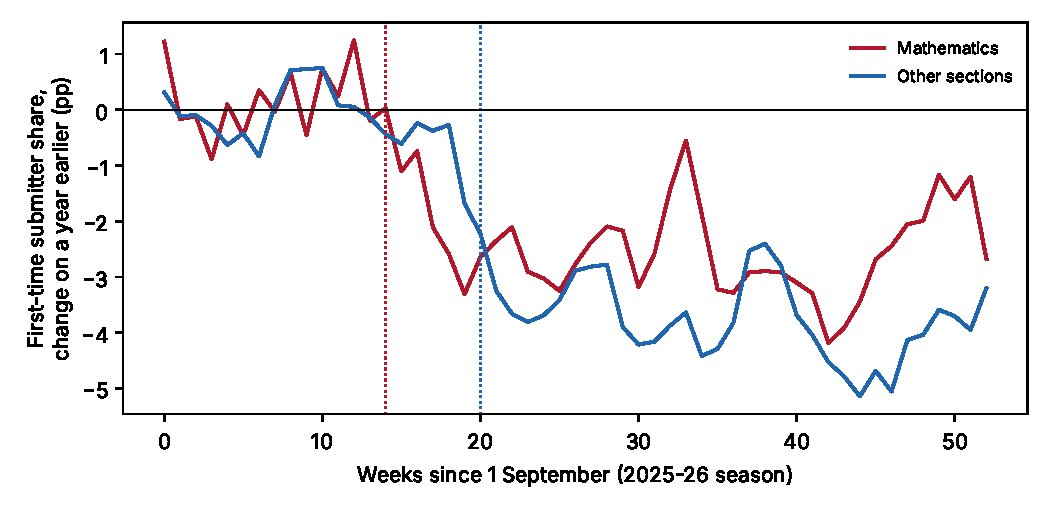
\includegraphics[width=\textwidth]{figures/emp_endorsement.pdf}
\caption{Endorsement rule}
\end{subfigure}\hfill
\begin{subfigure}{0.49\textwidth}
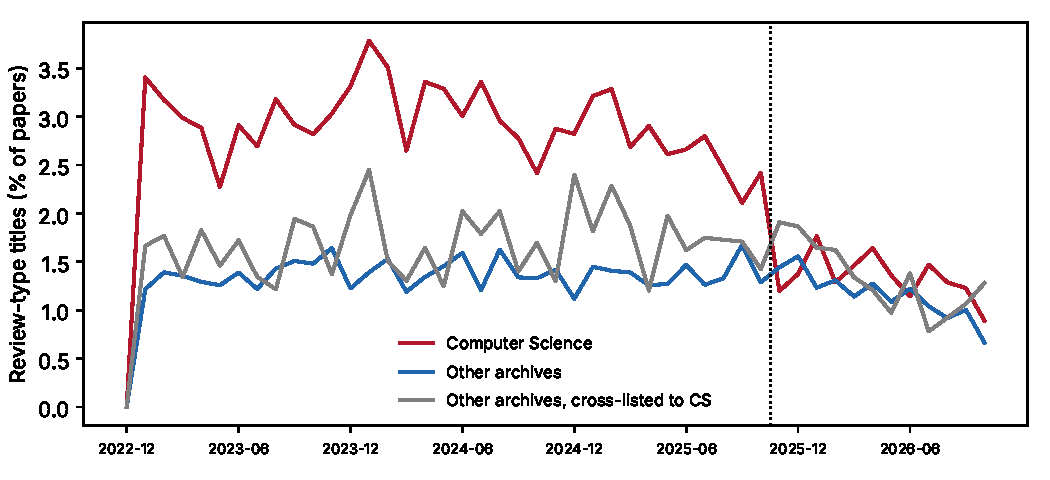
\includegraphics[width=\textwidth]{figures/emp_cs_reviews.pdf}
\caption{CS review policy}
\end{subfigure}
\caption{Two arXiv rule changes. (a) First-time submitter share, change on the same
week a year earlier (three-week moving average), Mathematics and other sections;
dotted lines mark 10 December 2025 and 21 January 2026. (b) Share of papers with
review-type titles by archive; the dotted line marks November 2025.}
\label{fig:policies}
\end{figure}

\begin{table}[p]
\centering\footnotesize
\caption{arXiv rule changes as shocks to entry, catch-up and writing}\label{tab:policies}
\resizebox{\textwidth}{!}{\begin{tabular}{@{}lrrl@{}}
\toprule
Design and outcome & Estimate & (SE) & Pre-period mean \\
\midrule
\multicolumn{4}{@{}l}{\emph{A. Endorsement tightening (entry cost): Mathematics 10 Dec 2025, all sections 21 Jan 2026}} \\
First-time submitter share, Mathematics, vs.\ year before & $-0.024$ & $(0.003)$ & 0.141 \\
First-time submitter share, other sections, vs.\ year before & $-0.034$ & $(0.003)$ & 0.222 \\
First-time submitter share, Mathematics vs.\ others, 10 Dec--20 Jan & $-0.017$ & $(0.004)$ & \\
Submitters with no prior arXiv authorship, Mathematics & $-0.009$ & $(0.003)$ & 0.043 \\
Submitters with no prior arXiv authorship, other sections & $-0.009$ & $(0.002)$ & 0.054 \\
log number of first-time submitters, other sections & $-0.154$ & $(0.035)$ & \\
\midrule
\multicolumn{4}{@{}l}{\emph{B. Peer review required for CS review and position papers (catch-up cost), 31 Oct 2025}} \\
Review-type share of papers, CS vs.\ other archives & $-0.013$ & $(0.001)$ & 0.027 \\
\quad with a CS-specific linear trend & $-0.010$ & $(0.002)$ & \\
\quad leakage: non-CS primary cross-listed to CS & $-0.002$ & $(0.001)$ & \\
Within CS: change in review share on pre-period review share & $-0.41$ & $(0.10)$ & 0.027 \\
\quad placebo, one year earlier & $-0.13$ & $(0.09)$ & \\
Within CS: change in first-time-author share on review share & $-0.70$ & $(0.26)$ & \\
\quad placebo, one year earlier & $-0.32$ & $(0.17)$ & \\
\midrule
\multicolumn{4}{@{}l}{\emph{C. Two submissions per submitter per month (writing cap), 1 Oct 2026}} \\
Third-or-later submissions in days 1--15, single-field names: Jan--Sep 2026 & $1.66\%$ & & \\
\quad October 2026 (residual: shared names and proceedings accounts) & $0.38\%$ & & \\
log papers per weekday, Oct 1--15 vs.\ Sep 1--15: 2026 & $+0.220$ & & \\
\quad same change in 2024 and 2025 & $+0.173$, $+0.178$ & & \\
Category dose-response: change on exposure (vs.\ 2025) & $+0.03$ & $(2.95)$ & 0.016 \\
\midrule
\multicolumn{4}{@{}l}{\emph{D. Author-level adoption of LLM-style writing (drafting speed)}} \\
log(1 + papers per half-year), adopters vs.\ others, 2024--26, all fields & $+0.022$ & $(0.005)$ & 0.48 \\
\quad fields where AI is not the subject (no cs, stat, eess) & $+0.024$ & $(0.007)$ & 0.52 \\
\bottomrule
\end{tabular}
}
\par\smallskip
\begin{minipage}{\textwidth}\footnotesize
Notes: Panel A: weekly cells by announcement week, September 2024--October 2026;
each week is differenced against the same week a year earlier; Newey--West
standard errors (four lags). Panel B: monthly cells, 2023--2026, archive and month
fixed effects, robust standard errors; dose-response across 29 CS categories with
at least 300 papers a year, weighted by size, Nov--Oct years. Panel C: days 1--15
of each month, papers announced in their regular batch; exposure is the
category's Jan--Sep 2026 share of excess submissions. Panel D: submitter and
field-by-half-year fixed effects, standard errors clustered by submitter.
Identities are name keys throughout (\cref{app:data}).
\end{minipage}
\end{table}

\subsection{What the shocks say about the model}

The four designs do not test every proposition, and two of them are first
stages whose outcomes are still accruing. Together they establish three
things. The entry margin responds to its cost, which is what makes density
respond little to volume. The supply of review articles, a lever on catch-up
costs, responds to policy, and the first reduced form on entry has the sign the
model predicts. And the detection of overlapping work does not run through
passive visibility. Reading protects through deliberate search, which is why
better search tools, not more prominent announcements, are the channel through
which AI could move the aware share. A per-person writing cap, finally, is not a
lever on volume at all.

\section{Quantification}\label{sec:quant}

This section puts numbers on the mechanisms. The aim is not to fit every
moment of the arXiv record. It is to check that one parameterisation of the
model reproduces the main facts with plausible primitives, and to read off its
implications for rents, the speed limit, the incidence of research tools,
topic life cycles and growth.

\subsection{Strategy}

We use the functional forms of \cref{sec:model}: harmonic learning
\eqref{eq:Qexample}, exponential detection and the exact catch-up time
\eqref{eq:T}. Time is measured in years. \Cref{tab:calibration} lists the
parameters. Some are set externally. The unit of density is fixed by $b=100$
papers read per year at full-time reading, and production speed by $a=4$
projects per year at full-time production. Careers leave a topic at $\rho=0.10$
(ten-year tenure), the stock's relevance decays at $\delta=0.25$ (a half-life of
about three years), topics become obsolete at $\xi=0.04$, and a newborn topic
produces $P_0=2$ papers a year. The credit block comes from
Fact~\ref{fact:credit} through \cref{lem:credit}. With exponential follow-on
credit and a pivot that costs 30\% of a project, the $+29\%$ premium of aware
follow-ons and the $-19\%$ penalty of unaware duplicates imply that 31\% of
detected overlaps proceed and that detection averts $\Delta/\lambda=37\%$ of
erosion. We set concurrent overlap to zero: our moments do not separate it from
erosion by unread earlier work, and attributing all erosion to unread work
gives reading its largest protective value. Explorers found a viable topic at
rate $s=0.14$, so that half of them found one before their spell ends
($\omega=1/2$). The frontier block splits the calibrated frontier value into
exploration and founding; it does not affect the cross-section, and we report
results for $\omega$ between 0 and 3/4.

The remaining parameters are calibrated jointly: learning ($\beta,\gamma$),
erosion ($\theta\lambda$), search precision ($\sigma$), the frontier value $F$,
catch-up speed $b_c$, and the distributions of diffusion rates and fertility.
The targets are the corrected returns profile of Fact~\ref{fact:hump}: the
gradient per standard deviation of density, the returns of the sparsest,
fourth and densest fifths relative to the middle one ($-11\%$, $+2\%$, $-2\%$),
and the 12\% of researcher-years beyond the peak. We add the recall-corrected
aware share of 60\% at mature density (Fact~\ref{fact:aware}), which
disciplines $\sigma$, and the share of incumbents' time spent reading. Faculty
report about 144 hours a year reading scholarly articles
\citep{tenopirking2008}, about 7\% of a working year. This target disciplines
the time-share value of reading tools (\cref{lem:timeshares}), which the
previous version of the model left free. A soft target puts the incumbents'
log premium $(\rho+\xi)T$ at about 0.15, about a year of catch-up per
seven-year spell in a topic. Since the measured gradient also reflects
audience, this is generous to the catch-up channel. We simulate the stationary
cross-section of topic life cycles and run the arXiv regressions on it. As in
the data, density is measured with error. Only 58\% of a paper's nearest
neighbours fall in its own fine area. We add classical noise with a standard
deviation of 0.3 in log density, which implies a reliability of about 0.8.
Researchers who move between topics supply the identifying variation in an
author-fixed-effects design, and the model has no ability differences. The
baseline analogue is therefore the cross-section of researcher-years. The
within-topic analogue, which uses only life-cycle variation, is a robustness
check. The search is a quasi-random scan of 2,048 points followed by
Nelder--Mead from the best points and from the previous calibration, with the
winner selected on a fine simulation grid (\cref{app:numerics}). The frontier's
depletion $\eta_F$ is then set from \eqref{eq:eta} with $\mathcal E=0.15$
(Fact~\ref{fact:volume}).

\begin{table}[t]
\centering\small
\caption{Parameters}\label{tab:calibration}
\begin{tabular}{@{}llll@{}}
\toprule
Parameter & Meaning & Value & Source \\
\midrule
\multicolumn{4}{@{}l}{\emph{Set externally}} \\
$b$ & papers read per year at full-time reading & 100 & normalisation (unit of $P$) \\
$\lambda$ & credit lost by an unaware duplicate & 0.19 & Fact 3 ($-19\%$) \\
$\kappa_p$ & credit lost by pivoting & 0.30 & assumption \\
$\Delta/\lambda$, $q$ & detection value; share proceeding & 0.37, 0.31 & Fact 3 ($+29\%$), \cref{lem:credit} \\
$\delta$ & decay of the stock's relevance & 0.25 & half-life $\approx$ 2.8 years \\
$\rho$ & rate of leaving a topic & 0.10 & ten-year topic tenure \\
$\xi$ & topic obsolescence & 0.04 & 25-year topic life \\
$P_0$ & flow of a newborn topic & 2 & a few papers per year \\
\multicolumn{4}{@{}l}{\emph{Calibrated (\cref{tab:fit})}} \\
$\beta$, $\gamma$ & learning efficiency, curvature & 39.01, 0.156 & hump in returns \\
$\theta\lambda$ & erosion per earlier paper & 0.0041 & fall at the top \\
$F$ & frontier payoff & 1.768 & sparsest fifth \\
$b_c$ & catch-up reading speed & 25 & premium, share beyond peak \\
$\sigma$ & search precision & 1.58 & recall-corrected aware share \\
$g_{\rm med}$, $s_g$ & diffusion rate: median, log-sd & 0.182, 0.29 & share beyond peak, fifths \\
$s_\zeta$ & log-sd of topic fertility & 0.052 & gradient across topics \\
$\eta$ & frontier elasticity & 0.0067 & $\mathcal{E}=0.15$ (Fact 1), \eqref{eq:eta} \\
\bottomrule
\end{tabular}

\end{table}

\begin{table}[t]
\centering\small
\caption{Fit to the arXiv facts}\label{tab:fit}
\begin{tabular}{@{}lccc@{}}
\toprule
Moment & arXiv & Baseline & Within-topic \\
\midrule
Gradient per SD of density & 0.067 & 0.049 & 0.055 \\
Sparsest fifth vs.\ middle & -0.080 & -0.071 & -0.096 \\
Fourth fifth vs.\ middle & 0.050 & 0.035 & 0.023 \\
Densest fifth vs.\ middle & 0.010 & 0.067 & 0.028 \\
Researcher-years beyond the peak & 0.120 & 0.129 & 0.125 \\
Incumbents' log premium $\kappa P^m$ & 0.150 & 0.189 & 0.172 \\
Peak of $v$ (SD above mean)$^\dagger$ & 1.00 & 0.92 & 1.10 \\
Quadratic: linear term$^\dagger$ & 0.094 & 0.048 & 0.052 \\
Quadratic: squared term$^\dagger$ & -0.047 & -0.001 & -0.009 \\
Aware share of flagged overlap$^\dagger$ & 0.38 & 0.38 & 0.89 \\
\bottomrule
\end{tabular}

\par\smallskip\footnotesize
$^\dagger$ Not targeted. Baseline: cross-section of researcher-years (movers
across topics). Within-topic: topic fixed effects, recalibrated. Density is the
researcher-weighted standardised log flow, measured with noise as in the data.
The reading share is from \citet{tenopirking2008}.
\end{table}

\subsection{Fit}

\Cref{tab:fit} and \cref{fig:test4} compare model and data. The baseline
calibration reproduces the aware share at mature density (\calAware\ against
60\%), the reading share of incumbents' time (\calReadCS\ against 7\%), most of
the share of researcher-years beyond the peak of the payoff curve
(\calBeyond\ against 12\%) and most of the rise from the sparsest fifth
(\calQone\ against $-11\%$). Without targeting it, the peak lies \calZhat\
standard deviations above mean density, against about one in the data. The
gradient falls short (\calLin\ against 6.7\%), and so does the incumbents'
premium, which is generous to the catch-up channel because the measured
gradient also reflects audience. Exact catch-up makes the problem harder than
it was with the linear approximation: the newcomer's payoff curve now falls
about twice as steeply at the mature density, and fast topics stop well below
the densities they reached before, so the life cycle generates less
overshooting for a given distribution of diffusion rates.

The model still does not reproduce the top of the profile. In the corrected
data the densest fifth earns \emph{less} than the middle ($-2\%$). In the model
the fourth and densest fifths earn \calQfour\ and \calQfive. The source of the
miss is composition. The densest researcher-years in the model include the most
fertile mature topics, whose incumbents earn high returns, alongside the
overshooting topics that pull returns down. Erosion in mature topics is small,
about \calErosion\ of credit, so the payoff curve falls only gently beyond its
peak. The fall at the top points to crowding costs in dense topics beyond
duplication and catch-up, to concurrent overlap, which we set to zero, or to
audience effects that flatter the middle of the distribution. We regard it as
the model's main quantitative failure. \calShareMature\ of researcher-years are
in mature topics, \calShareCons\ in topics consolidating after a growth spurt or
declining after a stall, and \calShareGrowth\ in growing topics. The
within-topic calibration fits its moments more closely (\cref{tab:fit}). Its
median diffusion rate is low, \calWGmed\ a year, so young topics grow slowly and
the life-cycle variation it relies on is spread over many years; relaxing the
bounds of the search does not change it.

\begin{figure}[t]
\centering
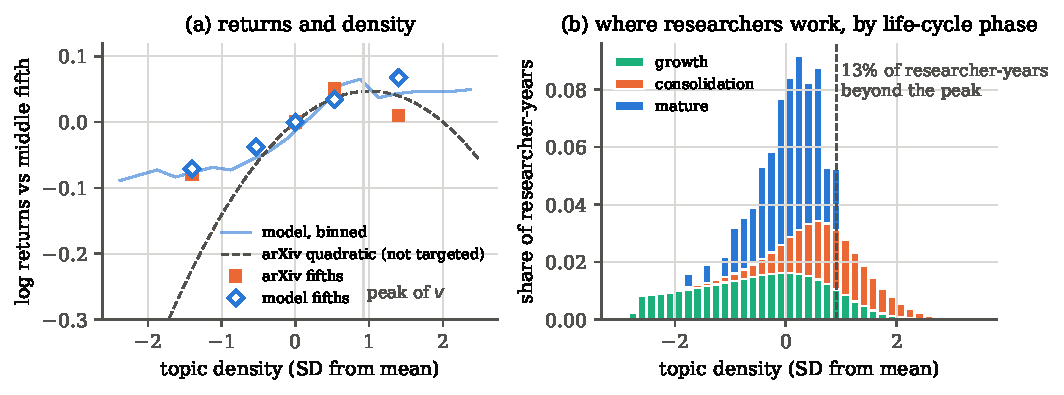
\includegraphics[width=\textwidth]{figures/fig4_test4.pdf}
\caption{Returns and density in the model. Left: log returns by observed (noisily
measured) topic density, relative to the middle fifth, in the calibrated
cross-section, with the arXiv fifths and the arXiv quadratic (not targeted).
Right: the distribution of researcher-years by true density and life-cycle phase.
Researcher-years beyond the peak of $v$ are concentrated in topics consolidating
after fast growth.}
\label{fig:test4}
\end{figure}

\subsection{What the calibrated model says}

\Cref{tab:welfare} collects the implications.

\begin{table}[t]
\centering\small
\caption{Rents, the speed limit, welfare and growth in the calibrated model}\label{tab:welfare}
\begin{tabular}{@{}lr@{}}
\toprule
Object & Value \\
\midrule
Peak of the payoff curve $\hat P$ (papers per year) & 23.4 \\
Gain from cumulative knowledge at the peak, $\hat v/v(P_0)-1$ & 17.0\% \\
Mature density $P^m$ & 12.0 \\
Catch-up time $T=S/b_c$ (years) & 1.68 \\
Incumbents' premium over the frontier, $e^{\kappa P^m}-1$ & 18.3\% \\
Rent at the peak, $\hat v/F-1$ & 20.1\% \\
Frictionless benchmark: rent dissipated, $1-F/\hat v$ & 16.7\% \\
Catch-up economy: planner's gain, $\hat w/F-1$ & 4.4\% \\
Optimal frontier subsidy, $s^o/F$ & 4.4\% \\
Overshooting threshold $g^*$ (per year) & 0.197 \\
Slope of the entrant payoff curve $|\varepsilon_w(P^m)|$ & 0.125 \\
Frontier elasticity $\eta$ (from $\mathcal{E}=0.2$) & 0.0328 \\
Stepping-on-toes parameter $\lambda_J=1-\mathcal{E}|\varepsilon_w|$ & 0.975 \\
\bottomrule
\end{tabular}

\end{table}

\paragraph{Rents and the speed limit.} The payoff curve peaks at
$\Phat=\calPhat$ papers a year, the newcomer's payoff curve at
$\hat P_w=\calPw$, and mature topics sit between them, at $P^m=\calPm$. The speed
limit is $b_c=\calBc$ papers a year: mature topics sit at \calSpeedRatio\ of it,
and the most fertile at \calSpeedRatioTop. Catching up takes \calT\ years at the
mature density and \calTpeak\ at the peak. Incumbents earn a premium of
\calPremium\ over the frontier, and the cross-topic returns gradient, the
catch-up elasticity $\eps_\Gamma=\calEpsG$, is steeper than the premium, as
\cref{prop:mature}(iv) requires. Even with rising incumbent returns
($\eps_v(P^m)=\calEpsV>0$), the newcomer's payoff curve is falling at the mature
density ($|\eps_w|=\calEpsW$), so mature topics are too crowded once the
catch-up burden is counted (\cref{cor:overcrowd}). Moving every topic to the
peak of $w$ raises output per researcher by \calPlannerGain\ (\calWPlannerGain\
in the within-topic calibration). The frictionless benchmark, in which catch-up
is free and topics fill to the density where $v=F$, would dissipate \calDissip\
of output per researcher. That number describes a counterfactual economy, not
the calibrated one.

\paragraph{The incidence of research tools.} \Cref{tab:ai,tab:incidence} and
\cref{fig:incidence} report the effects of 30\% improvements in each channel.
Reading takes \calRm\ of an incumbent's time at the mature density, so faster
reading is worth $r^*/(1-r^*)=\calTimeValueRead$ per log point at a fixed topic:
a 30\% faster reader gains \calReadFixed\ log points, a 30\% faster producer
\calWriteFixed. Per hour saved, the two are worth the same. Entry then ranks
them. The producer keeps almost everything, \calWriteOut\ log points. If
explorers never stay in the topics they open, the reader keeps
\calReadOutNoF\ log points, \calReadPassNoF\ of her gain, close to the floor
$\mathcal ED$ of \eqref{eq:passthrough}. If founders stay with probability one
half, she keeps \calReadOut, or \calReadPass. Per hour saved, a production tool
is therefore worth between \calPerHour\ and \calPerHourNoF\ times a reading
tool. Catch-up tools keep \calCatchPassNoF\ without founders and \calCatchPass\
with them; founders never catch up, so their gain reaches the frontier only
through the density of the topics founders end up in.

On the simulated life cycle the founders' channel is weaker for catch-up
tools and somewhat weaker for reading tools. Founders spend much of their
tenure in topics still growing at a pace set by diffusion, so the frontier
value rises by \calLCReadF\ of a reading gain and by only \calLCCatchF\ of a
catch-up gain. Output per researcher-year, which also counts the rents of
newcomers who enter growing topics before entry pays only the frontier value,
rises by more: \calLCReadY\ of a reading gain (\calLCReadYnoF\ without founders),
\calLCCatchY\ of a catch-up gain and \calLCProdY\ of a production gain. These
rents raise life-cycle output per researcher \calLCRent\ above the frontier
value. The footprints in \cref{tab:ai} follow \cref{prop:ai}. Faster reading
raises density by \calReadDens\ log points; faster catch-up raises it by
\calCatchDens\ and lowers the overshooting threshold by \calCatchGstar\
percentage points, so more topics grow too fast; better search raises the aware
share by \calSearchAware\ percentage points.

\begin{table}[t]
\centering
\caption{How much of each tool survives entry, and readership}\label{tab:incidence}
\small
\begin{tabular}{@{}lrrrrrr@{}}
\toprule
 & \multicolumn{2}{c}{Faster reading} & \multicolumn{2}{c}{Faster catch-up} & \multicolumn{2}{c}{Faster production} \\
\cmidrule(lr){2-3}\cmidrule(lr){4-5}\cmidrule(l){6-7}
 & formula & life cycle & formula & life cycle & formula & life cycle \\
\midrule
\multicolumn{7}{@{}l}{\emph{A. Share of the gain at fixed topics that survives entry (\%)}} \\
$\omega=0.00$ & 17 & 40 & 17 & 11 & 99 & 99 \\
$\omega=0.25$ & 50 & 44 & 31 & 17 & 99 & 99 \\
$\omega=0.50$ & 74 & 63 & 41 & 17 & 99 & 99 \\
$\omega=0.75$ & 91 & 79 & 48 & 16 & 99 & 99 \\
\midrule
\multicolumn{7}{@{}l}{\emph{B. Long-run gain valued by readership, $\omega=0.5$ (log points $\times100$)}} \\
$\alpha=0.0$ & \multicolumn{2}{c}{$+1.5$} & \multicolumn{2}{c}{$+1.0$} & \multicolumn{2}{c}{$+26.0$} \\
$\alpha=0.5$ & \multicolumn{2}{c}{$+11.3$} & \multicolumn{2}{c}{$+6.3$} & \multicolumn{2}{c}{$+13.6$} \\
$\alpha=1.0$ & \multicolumn{2}{c}{$+21.2$} & \multicolumn{2}{c}{$+11.5$} & \multicolumn{2}{c}{$+1.3$} \\
\bottomrule
\end{tabular}
\par\smallskip\footnotesize Panel A: \emph{formula} is the frontier-incidence pass-through at the mature density (\cref{thm:incidence}) with founders' topics valued at maturity and $\eta_F$ set from the volume elasticity; \emph{life cycle} re-solves the founders' fixed point $F=(1-\omega)e+\omega\bar U_F(F)$ on the simulated life cycle (no depletion) and measures output per researcher-year with exploration, catch-up and diffusion rents counted. Panel B: output valued as $A^\alpha Y$, where $A=(b/a)r^*/(1-r^*)$ is reads per paper; $\alpha=0$ is credited output, $\alpha=1$ readership.

\end{table}

\begin{figure}[t]
\centering
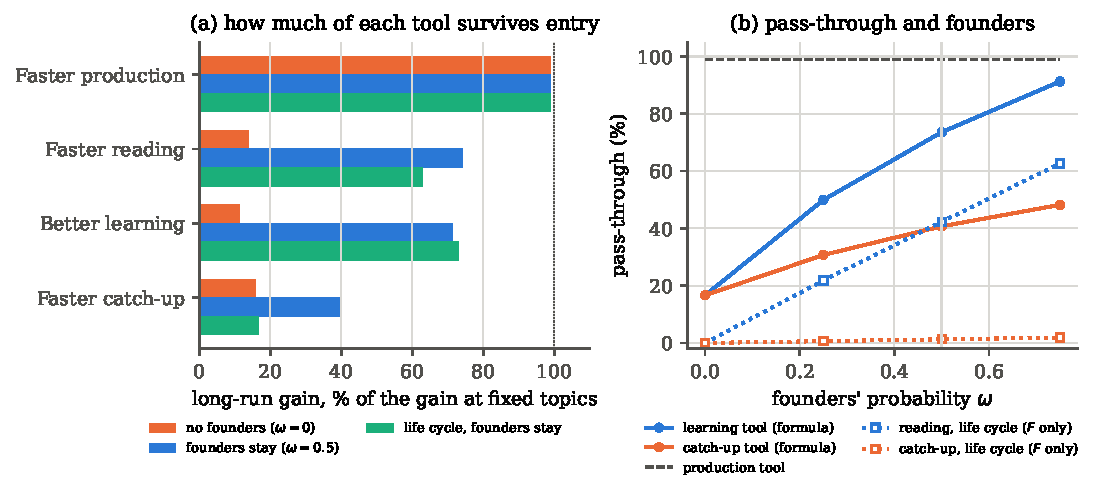
\includegraphics[width=\textwidth]{figures/fig5_incidence.pdf}
\caption{The incidence of research tools in the calibrated model (30\% shocks).
Left: long-run gain in output per researcher as a share of the gain at fixed
topics, without founders, with founders who stay (stationary), and on the
simulated life cycle. Right: the share that survives entry as a function of
the founders' probability $\omega$, from the incidence formula and, for the
frontier value alone, on the life cycle.}
\label{fig:incidence}
\end{figure}

\paragraph{Readership.} Valued by readership ($\alpha=1$ in
\cref{prop:audience}), a 30\% faster pen adds \calAudWrite\ log points and 30\%
faster reading \calAudRead: a faster pen leaves total reading unchanged and
cuts reads per paper by \calReadsDrop. With readership given half the weight of
credit ($\alpha=1/2$) the two tools are worth about the same, \calAudWriteHalf\
and \calAudReadHalf\ log points. Which tool scales science depends on the unit,
and the unit is a choice about what science values.

\paragraph{Topic life cycles.} A newborn topic beats the frontier by
\calNewborn, so its first followers join, but a stationary topic of the same
density would not be worth joining. Topics that grow more slowly than
\calGtakeoff\ a year stall in the valley and are abandoned, and topics that grow
faster than \calGstarExact\ overshoot the peak (\cref{prop:toofast}); with
foresight the overshooting threshold is \calGstarRE. These are fast but not
unusual rates for hot topics on arXiv.

\paragraph{Growth.} Inverting \eqref{eq:eta} with $\mathcal E=0.15$ gives a frontier
depletion of $\eta_F=\calEta$ (\calEtaNoF\ without founders), and the
stepping-on-toes parameter is $\lambda_J^{\rm eq}=1-\mathcal E|\eps_w|=\calLambda$ when
topics adjust and $\lambda_J^M=1+\eps_w/D=\calLambdaFixed$ when open topics are
held fixed (\cref{prop:sot}). Over the arXiv range $\mathcal E\in[0,0.27]$,
$\lambda_J^{\rm eq}$ lies between \calLambdaLo\ and one. The short-run bias from
topic-age composition (\cref{rem:shortrun}) is $-\calCompBias$ over a
seven-year window, so even the upper end of the long-run range keeps
$\lambda_J^{\rm eq}$ close to one. Topic crowding and access depletion explain
little of the diminishing returns to research found by \citet{bloometal2020}.
Their estimates require $\lambda_J$ well below one, which in our framework must
come from fertility depletion (\cref{app:fertility}) or from selection.

\section{Aggregate implications}\label{sec:macro}

\subsection{Stepping on toes, measured}

Growth models since \citet{jones1995} let the flow of new ideas scale with
researchers as $N^{\lambda}$, $\lambda<1$, and call $1-\lambda$ ``stepping on
toes''. The parameter is reduced form. Here the flow of credited novel output
is $Y=N\,a\,F(M^*(N))$, because in equilibrium every researcher's career payoff
equals the frontier's. The model therefore gives $\lambda$ as an equilibrium object.

\begin{proposition}[Stepping on toes]\label{prop:sot}
In the large-topic limit,
\begin{equation}\label{eq:sot}
\lambda\equiv\frac{\dd\ln Y}{\dd\ln N}=1-\eta\,\frac{\dd\ln M^*}{\dd\ln N}=1-\mathcal E\,|\eps_w(P^*)|.
\end{equation}
If, in addition, topics opened later are less fertile, with fertility elasticity $\eta_f\ge0$ (\cref{app:fertility}), the right-hand side of \eqref{eq:sot} is an upper bound on $\lambda$.
\end{proposition}

The formula is a sufficient statistic built from two observable objects. The
first is the volume elasticity of density, $\mathcal E$ (Test 1). The second is
the elasticity of the entrant's payoff curve at equilibrium density, $\eps_w=\eps_v-\kappa P^*$. That is the
incumbent's returns gradient minus the catch-up premium (Test 4 and
\cref{prop:mature}). Crowding does not \emph{amplify} frontier depletion, as
the draft conjectured. It \emph{buffers} it. The density margin absorbs part of
the growth in researchers, so fewer new topics are opened and the frontier
deteriorates more slowly. The cost of crowding shows up in the \emph{level} of
productivity, as the dissipated rent $\hat w-F$, and not in its elasticity.
With $\mathcal E\approx0.2$ and the calibrated slope of $w$, crowding and access
depletion together imply $\lambda$ close to one (\cref{sec:quant}). The bulk of the measured
decline in research productivity \citep{bloometal2020} must come from
elsewhere: falling fertility of new topics ($\eta_f$, not identified by density
data) or selection on researcher ability, as in \citet{ekerdtwu2024}.

\subsection{A Solow paradox for science}

The last half-century brought enormous improvements in access to the
literature: online journals, preprint servers, full-text search, and now
language models that read for us. Measured research productivity fell
throughout \citep{bloometal2020}. \Cref{prop:ai}(iii) suggests one reason.

\begin{proposition}[Reading improvements are dissipated]\label{prop:solow}
Let $\omega$ be any parameter that raises $w$ at every density and leaves $F$
unchanged. In the large-topic limit, $\dd P^*/\dd\omega>0$ and
$\dd M^*/\dd\omega<0$, and
\[
\frac{\dd\ln(Y/N)}{\dd\omega}=\eta\left|\frac{\dd\ln M^*}{\dd\omega}\right|\ge0,
\]
with equality if and only if $\eta=0$. By contrast, $\dd\ln(Y/N)/\dd\ln a=1-\mathcal E|\eps_w|$.
\end{proposition}

Better access to knowledge raises the payoff of working in existing topics.
Newcomers respond by crowding them until they are no better than the frontier.
What remains is denser topics, fewer new ones, and the same output per
researcher. The prediction matches \citet{evans2008}, who finds that online
access narrowed the set of papers that get cited. It also matches
\citet{haoetal2026}, who find that AI tools ``contract science's focus''. Gains
from access to frontier knowledge measured at the level of individuals or
topics \citep{iariaetal2018,biasimoser2021} are real, but in equilibrium they
are partly competed away at the level of science.

\section{Out-of-sample predictions}\label{sec:predictions}

The catch-up extension was added after the returns-by-density evidence was
seen, so that evidence cannot test it. The predictions below were not used to
build the model. They are stated before the relevant data were analysed, and
several before the data exist. To make the claim verifiable they should be
deposited in a public registry before they are taken to the data. The
replication package contains the text.

\paragraph{Predictions testable with existing data.}
\begin{enumerate}[label=\textbf{P\arabic*.},leftmargin=*]
\item \emph{Overcrowding is young and fast.} The fall in returns beyond the peak
should be concentrated in clusters whose flow grew faster than their stock, that
is, with a high flow-to-stock ratio $P/S$ (\cref{prop:toofast}). Among mature
clusters the returns curve should be monotone.
\item \emph{Slow clusters die young.} Among clusters born in the same year, those
whose flow grew slowly in their first years should be abandoned more often, and
the hazard should fall sharply above a threshold growth rate
(\cref{prop:toofast}(i)).
\item \emph{Returns follow the stock, density follows the flow.} Holding flow
density fixed, returns should rise with the cluster's depreciated stock of
literature (\cref{prop:mature}(ii): the premium is $(\rho+\xi)T(P,S)$).
\item \emph{Newcomers start slowly where stocks are large and flows are fast.}
The lag between a newcomer's arrival in a cluster and her first paper there, and
the length of her first reference list, should rise with the cluster's stock,
and convexly with its flow as the flow approaches what newcomers can read
(\cref{lem:career}). Incumbents should show no such gradient.
\item \emph{The cross-topic gradient is the catch-up elasticity plus audience.}
The returns gradient from researchers who switch clusters should exceed the log
premium of incumbents over pioneers in the clusters they join, by the gap
between the catch-up elasticity and the premium (\cref{prop:mature}(iv)) and by
the audience effect, which can be measured with citations from outside the
cluster.
\item \emph{Close overlap is pinned; broad neighbourhoods fill.} The volume
elasticity should rise with the similarity radius, from near zero at the overlap
radius toward the fixed-field benchmark at broad radii (Fact~\ref{fact:volume}
already shows this ordering), and the ordering should survive embedding-based
similarity. The ratio of the two elasticities measures how easily topics open
inside existing fields (\cref{prop:nested}).
\item \emph{Founders stay.} The share of a cluster's founding authors who keep
publishing in it, and their returns there relative to their earlier exploratory
work, measure the founders' share of the frontier's value, $\theta_F$. Areas with
a larger $\theta_F$ should gain more from reading tools (\cref{thm:incidence}).
\item \emph{Stepping on toes across areas.} Areas with a larger volume elasticity
of density should show stronger diminishing returns to researchers in citation
output, with $1-\lambda_J^{\rm eq}=\mathcal E|\eps_w|$ area by area
(\cref{prop:sot}).
\item \emph{Search costs and detection.} Google was blocked in mainland China
from 2014 \citep{zhengwang2020}. Relative to Hong Kong-based and overseas
Chinese authors in the same topics, mainland-based authors' close overlaps
should have become less often aware, and their papers more often unaware
duplicates, after 2014 (\cref{lem:credit} with lower $\sigma$). The share of
covering papers they pivot away from cannot be observed, so the prediction is
on the aware share and on the citation penalty of their overlaps.
\end{enumerate}

\paragraph{Predictions for the arXiv rule changes of 2025--2026.}
\begin{enumerate}[label=\textbf{P\arabic*.},leftmargin=*,resume]
\item \emph{Endorsement.} Relative to the other sections, Mathematics in
2026 and all sections in 2026--2027 relative to trend should show fewer pioneer
papers (new clusters) in proportion to the fall in entrants. Local density at
the overlap radius, the flagged overlap rate and the aware share should not
change detectably (\cref{prop:ai}(ii) with small $\mathcal E$).
\item \emph{Review articles.} In computer-science clusters where reviews had been
common, mature density should fall and the number of clusters rise relative to
other computer-science clusters over 2026--2027. Fast-growing clusters there
should overshoot less (higher $g^*$) and newcomers' first papers should come
later and with longer reference lists (\cref{prop:ai}(iv), P3).
\item \emph{Submission cap.} The cap should leave total volume, papers per
author and the overlap rate within a few percent of trend. Submissions by
previously heavy submitters should be replaced partly by submissions in their
co-authors' names.
\item \emph{Reading tools.} When literature-summarising tools are widely used,
high-uptake fields where AI is not the subject should form fewer new clusters,
thicken existing ones, and show more overshooting by fast-growing clusters.
Overlap measured by meaning should rise in dense clusters, and citations per
author-year should rise by much less than the time the tools save, except where
the people who open new clusters use them (\cref{prop:ai}(iii)--(iv),
\cref{thm:incidence}).
\item \emph{Production shocks and closure.} A large, fast rise in production
speed should raise the flow of the densest clusters most, lengthen newcomers'
time to first paper there, and cut entry into them for a while
(\cref{thm:speed}(iv)).
\item \emph{Better search raises the aware share.} If search tools improve, the
share of close overlaps that cite the earlier paper should rise, with no
offsetting fall in the overlap rate in sparse clusters (\cref{prop:ai}(v)).
\end{enumerate}

Two earlier predictions have already been settled. Equal returns (full
dissipation) is rejected, and the catch-up cost replaces it. A detection
channel that runs through the prominence of a paper's announcement is rejected
by the listing-rank design (\cref{sec:causal}), which locates detection in
deliberate search.

\section{Conclusion}\label{sec:conclusion}

Is innovation too fast? The model's answer is that the question is usually asked about
the wrong margin. When papers arrive faster than they can be read, researchers do
not keep piling into the same topics until duplication explodes. They spread
out, and the overlap rate stays where entry pins it. The arXiv record bears this
out: the volume of papers more than doubled while close overlap barely moved.
The costs of speed lie elsewhere. The gains from building on others' work are competed away.
Incumbents keep rents behind a wall of reading that newcomers must climb.
Returns rise with density even though topics are too crowded at the margin.
And topics whose literature grows faster than newcomers can catch up overshoot.
Literally, they are too fast.

Several simplifications deserve scrutiny in future work. Credit is measured by
citations, which also reward audience size. This biases measured returns toward
dense topics, so the overcrowding we find is, if anything, understated.
Newcomers value topics at their current state, and diffusion rates are
exogenous. Forward-looking entry into a growing topic would anticipate
crowding and dampen overshooting, while information cascades would amplify it.
Topics are identical up to fertility. Their spatial arrangement in an area's
idea space appears only in prediction P7. And the frontier is a reduced-form
lottery. Endogenising it, for instance by letting pioneers choose how far from
existing topics to locate, is the natural next step. It is also the margin
that the policy conclusion below hinges on.

The policy implications follow from where the rents go. Anything that improves the payoff of
working inside existing topics is competed away. That includes better reading
tools, search engines, summarisers and caps on writing. Anything that improves
the frontier is not. Writing tools scale science because they scale the frontier
too. Reading tools crowd it unless they also make new topics easier to open. To
date, artificial intelligence has changed science mainly by lowering the cost of
entry, and the new entrants have spread out. The model predicts what will happen when tools that read for
us become widespread: denser topics, fewer new ones, more hot topics that
overshoot, and little gain in output per researcher. Unless, that is, the same
tools are pointed at the frontier.


\bibliographystyle{plainnat}
\bibliography{references}

\appendix
\section{Proofs}\label{app:proofs}

Throughout, ``concave'' means concave on the stated convex domain, and
$\partial_R$, $\partial_P$ denote partial derivatives.

\paragraph{The example satisfies \cref{ass:Q,ass:phi}.} The function
$h(R,P)=RP/(R+P)$ is half the harmonic mean of $R$ and $P$. It is concave,
nondecreasing and homogeneous of degree one on $\R_+^2$, with $h\le\min\{R,P\}$.
So $\ln(1+\beta h)$ is concave as a nondecreasing concave transformation of a
concave function, and $Q$ is bounded by $(1+\beta R)^\gamma$ for fixed $R$.
Supermodularity: $\partial_R\ln Q=\gamma\beta h_R/(1+\beta h)$ with
$h_R=P^2/(R+P)^2$ and $h_{RP}=2RP/(R+P)^3$, so
\[
\partial_P\partial_R\ln Q=\gamma\beta\,\frac{h_{RP}(1+\beta h)-\beta h_Rh_P}{(1+\beta h)^2}
=\gamma\beta\,\frac{2RP(R+P)+\beta R^2P^2}{(R+P)^4(1+\beta h)^2}\ge0 .
\]
For $\varphi(c)=1-e^{-\sigma c}$: $\varphi(0)=0$, $\varphi'=\sigma e^{-\sigma c}>0$, $\varphi''<0$.

\paragraph{Proof of \cref{lem:credit}.} Covering papers form a Poisson count
$K$ with mean $\theta P$. Each is detected independently with probability
$\varphi$, so detected and undetected counts $K_d,K_u$ are independent Poisson
with means $\theta P\varphi$ and $\theta P(1-\varphi)$. Credit is the product
of $(1-\lambda)$ over undetected papers and of independent factors with mean
$1-\ell$ over detected papers. Using $\E[t^{K}]=e^{-\mu(1-t)}$,
\[
C=\E\big[(1-\lambda)^{K_u}\big]\,\E\big[(1-\ell)^{K_d}\big]
=e^{-\theta P(1-\varphi)\lambda}\,e^{-\theta P\varphi\ell}
=\exp\{-\theta P[\lambda-(\lambda-\ell)\varphi]\}.
\]
Flagged overlap consists of undetected covering papers (rate $\theta
P(1-\varphi)$) and detected ones that proceed (rate $\theta P\varphi q$). The
aware share is the ratio of the second rate to the sum. Proceeding happens iff
$\delta>1-\kappa_p$, which gives the conditional mean. \qed

\paragraph{Proof of \cref{lem:career}.} Let careers end at rate $\rho$. A
newcomer to a stationary topic reads for $T=S/b_c=P/(\delta b_c)$ periods and
then earns $a\,v(P)$ until her career ends. Her expected career value is
$\int_T^\infty e^{-\rho t}a\,v(P)\,\dd t=a\,v(P)e^{-\rho T}/\rho=a\,w(P)/\rho$.
An explorer's value is $aF(M)/\rho$. In a stationary topic with entry flow
$e$, the mass of members in catch-up is $e(1-e^{-\rho T})/\rho$ and the mass
writing is $e\,e^{-\rho T}/\rho$. So the writing share of members is
$e^{-\kappa P}$, output per member is $a\,v(P)e^{-\kappa P}$, and \eqref{eq:flow}
gives $P=a\,x^*(P)\,n\,e^{-\kappa P}$. \qed

\paragraph{Proof of \cref{thm:v}.}
\emph{(i)} Since $Q(0,P)=1$ and $\varphi(0)=0$, $v(P)\ge g(0,P)=e^{-\theta\lambda P}$. Because $Q$ and $\varphi$ are nondecreasing in $R$ and $R\le b$,
\[
g(r,P)\le \bar Q(b)\exp\{-\theta P[\lambda-\Delta\varphi(b/P)]\}\xrightarrow[P\to\infty]{}0,
\]
since $\varphi(b/P)\to0$ and $\lambda>0$. At $P=0$, $g(r,0)=1-r$, so $v(0)=1$. Define $\ln C(R,0)=0$. Then $|\theta P\varphi(R/P)|\le\theta P$ gives joint continuity of $g$ on $[0,1]\times\R_+$ ($g\to0$ as $r\to1$). Berge's maximum theorem gives continuity of $v$.

\emph{(ii)} On $D=[0,1)\times(0,\infty)$,
\[
\ln g(r,P)=\ln(1-r)+\ln Q(br,P)-\theta\lambda P+\theta\Delta\,P\varphi\!\left(\frac{br}{P}\right).
\]
The first term is concave in $r$. The second is concave by \cref{ass:Q}
composed with a linear map. The third is linear. In the fourth, $(R,P)\mapsto
P\varphi(R/P)$ is the perspective of the concave function $\varphi$, which is
jointly concave on $\R\times\R_{++}$ \citep[\S3.2.6]{boydvandenberghe2004}. So
$\ln g$ is jointly concave on $D$. Since $\ln g\to-\infty$ as $r\to1$, the
supremum over $r$ is attained in $[0,1)$. Partial maximisation of a jointly
concave function over a convex set preserves concavity
\citep[\S3.2.5]{boydvandenberghe2004}. Hence $\ln v(P)=\max_r\ln g(r,P)$ is concave.

For strict concavity, take $P_1\neq P_2$ with maximisers $r_1,r_2$ and $t\in(0,1)$. Under \cref{ass:interior}(a), $\partial_r\ln g(0,P)>0$, so $r_i>0$. If $r_1\neq r_2$, strict concavity of $\ln(1-r)$ gives
$\ln g(r_t,P_t)>t\ln g(r_1,P_1)+(1-t)\ln g(r_2,P_2)$. If $r_1=r_2=r>0$, then $P\mapsto P\varphi(br/P)$ has second derivative $\varphi''(br/P)(br)^2/P^3<0$, which gives the same strict inequality. In either case $\ln v(P_t)\ge\ln g(r_t,P_t)>t\ln v(P_1)+(1-t)\ln v(P_2)$.

\emph{(iii)} Fix $\varrho$ with $\nu_0(\varrho)>0$. For small $P$, $r=\varrho P/b$ is feasible and
\[
\frac{v(P)-1}{P}\ge\frac{g(\varrho P/b,P)-1}{P}
=\frac{(1-\varrho P/b)\,Q(\varrho P,P)\,e^{-\theta P[\lambda-\Delta\varphi(\varrho)]}-1}{P}\longrightarrow \nu_0(\varrho)>0 .
\]
So $v>1=v(0)$ on some interval $(0,\epsilon)$. A strictly log-concave function is strictly quasi-concave, so its maximiser is unique. It is positive because $v$ exceeds $v(0)$ near zero, and finite because $v\to0$. Strict quasi-concavity gives strict monotonicity on either side of $\Phat$. Since $v$ falls continuously and strictly from $\vhat$ to $0$ on $[\Phat,\infty)$, each $F\in(0,\vhat)$ has exactly one root there.

\emph{(iv)} For $P>0$ the maximiser $r^*(P)$ is unique (strict concavity in $r$) and $\partial_P g$ is continuous. The envelope theorem \citep{milgromsegal2002} gives $v'(P)=\partial_Pg(r^*(P),P)$. Differentiating $\ln C$,
\[
\partial_P\big[-\theta\lambda P+\theta\Delta P\varphi(R/P)\big]=-\theta\lambda+\theta\Delta\big[\varphi(c)-c\varphi'(c)\big],\qquad c=R/P,
\]
which is \eqref{eq:envelope}. Concavity and $\varphi(0)=0$ give $\varphi(c)-c\varphi'(c)\ge0$.

\emph{(v)} $\partial_r\partial_P\ln g=b\,[\partial_R\partial_P\ln Q+\partial_R\partial_P\ln C]$. The first term is nonnegative by \cref{ass:Q}. For the second,
$\partial_R\ln C=\theta\Delta\varphi'(R/P)$, so $\partial_P\partial_R\ln C=-\theta\Delta\varphi''(c)\,c/P\ge0$. So $\ln g$ has increasing differences in $(r,P)$, and the unique maximiser is nondecreasing by Topkis's monotonicity theorem \citep{topkis1998}. \qed

\paragraph{Proof of \cref{prop:externality}.} By \cref{thm:v}(iv), the effect
of a marginal paper on an incumbent's per-period payoff is $a\,v'(P)$. Its sign is
that of $\Phat-P$ by \cref{thm:v}(iii). \qed

\paragraph{Proof of \cref{prop:eq}.} With $\kappa=0$, $n(P)=P/(a x^*(P))$ is
continuous and strictly increasing, since $x^*$ is nonincreasing by
\cref{thm:v}(v). Let $M(P)$ solve $\Phi(M)+Mn(P)=N$. It is unique,
continuous and strictly decreasing in $P$ ($\Phi$ is increasing). Define
$\Psi(P)=\ln v(P)-\ln F(M(P))$ on $[\Phat,\infty)$. $\ln v$ is strictly
decreasing there, and $F(M(P))$ is nondecreasing because $F$ is nonincreasing,
so $\Psi$ is strictly decreasing. In the large-topic limit $M(\Phat)=N/n(\Phat)$
and $\Psi(\Phat)>0$ by assumption. As $P\to\infty$, $v\to0$ while
$F(M(P))\ge F(M(\Phat))>0$, so $\Psi<0$ eventually. Hence there is a unique root
$P^*>\Phat$. Crossings on $(0,\Phat)$ violate stability, since there $v'>0$.
Payoff per researcher is $a\,v(P^*)=aF(M^*)<a\vhat$. \qed

\paragraph{Proof of \cref{prop:volume}.} In the large-topic limit
$M=N/n(P)=N\,a\,x^*(P)e^{-\kappa P}/P$, so the equilibrium condition
$w(P)=F\big(N a x^*(P)e^{-\kappa P}/P\big)$ involves $N$ and $a$ only through
$Na$. Log-differentiating with respect to $\ln N$,
\[
\eps_w\,\dd\ln P=-\eta\,[\dd\ln N-D\,\dd\ln P],\qquad D=\frac{\dd\ln n}{\dd\ln P}=1-\eps_x+\kappa P .
\]
Solving gives \eqref{eq:E}. Then $\dd\ln M=\dd\ln N-D\,\dd\ln P$, and papers per
researcher $a\,x^*(P)$ move with elasticity $\eps_x\,\mathcal E$. If $\eta=0$,
$P^*$ solves $w(P)=\bar F$, which involves neither $N$ nor $a$. The overlap rate
and the aware share are functions of $P^*$ by \cref{lem:credit}. Free entry into
science changes $P^*$ only through $N$. The general (non-limit) version
replaces $D$ by $D\,(1-s_e)$ and $|\eps_w|$ by $|\eps_w|[1+s_e(\phi_e-1)]$,
where $s_e=\Phi(M)/N$ and $\phi_e=M\Phi'(M)/\Phi(M)$. \qed

\paragraph{Proof of \cref{prop:planner}.} Write $D=1-\eps_x+\kappa P$; as
above $n\,\dd P/\dd n=P/D$. The Lagrangian
$a[f_0M+Mn\,w(P(n))]-\mu[\Phi(M)+Mn-N]$ has first-order conditions
\[
\mu=a\,w\Big(1+\frac{\eps_w}{D}\Big)\quad(n),\qquad a(f_0+nw)=\mu\Big(\frac1{\pi}+n\Big)\quad(M),
\]
using $\Phi'(M)=1/\pi(M)$. Eliminating $\mu$ and using $F=f_0\pi$ gives
\eqref{eq:plannerfoc}. Along the resource constraint,
$\dd n/\dd M=-(1/\pi+n)/M$, so
\[
\frac{\dd Y}{\dd M}=a(f_0+nw)-a\,w\Big(1+\frac{\eps_w}{D}\Big)\Big(\frac1\pi+n\Big).
\]
At the equilibrium ($w=F=f_0\pi$, $\eps_w<0$) this equals
$-a\,f_0(\eps_w/D)(1+n\pi)>0$. The planner therefore opens more topics, and
density falls below $P^*$. At $\hat P_w$ ($\eps_w=0$) it equals
$a f_0(1-w/F)<0$ whenever $w(\hat P_w)>F$. So the optimum lies in
$(\hat P_w,P^*)$. For (ii), the left side of \eqref{eq:plannerfoc} is bounded
by $(\hat w-F)/\hat w$ while $1+n\pi\to\infty$,
so $|\eps_w(P^o)|\to0$ and $P^o\to\hat P_w$ by strict log-concavity of $w$. For
(iii), with a subsidy $s$ to explorers the equilibrium condition becomes
$w(P)=F(M)+s$, and $s=s^o$ makes $(P^o,M^o)$ satisfy it. For (iv), let the
planner also set $x$. Per-member output is $a\,g(x,P)e^{-\kappa P}$, and at
fixed $n$, $\partial\ln P/\partial\ln x=1/(1+\kappa P)$. The first-order
condition for $x$ is
\[
\partial_x\ln g+\big[\partial_P\ln g-\kappa\big]\frac{P}{x(1+\kappa P)}=0 .
\]
At the private optimum $\partial_x\ln g=0$ and, by the envelope theorem,
$\partial_P\ln g-\kappa=(\ln w)'(P)$. The wedge therefore has the sign of
$(\ln w)'$. In the large-topic limit the planner maximises $\max_{x,P}g(x,P)e^{-\kappa P}=\max_P w(P)$. The maximum is at $(x^*(\hat P_w),\hat P_w)$, where the wedge is zero. \qed

\paragraph{Proof of \cref{prop:mature}.} (i) $\ln w=\ln v-\kappa P$ is strictly concave. Since $(\ln w)'(\Phat)=-\kappa<0$, the peak of $w$ lies below $\Phat$. (ii) The equilibrium condition and stability are those of \cref{def:eq}. The premium follows from $v(P^m)e^{-\kappa P^m}=F$ and $\kappa P=\rho T$. (iii) $P^m<\Phat$ iff $w(\Phat)<F$, since $w$ is falling on $(\hat P_w,\infty)$; this reads $\ln\vhat-\kappa\Phat<\ln F$. (iv) From $\ln\zeta+\ln v(P^m)=\ln F+\kappa P^m$, differentiate with respect to $\ln P^m$. \qed

\paragraph{Proof of \cref{cor:overcrowd}.} Total member output in a topic is $n\,a\,w(P(n))$, so one more member changes the output of the others by $n\,a\,w'(P)\,\dd P/\dd n$. Here $\dd P/\dd n>0$ and $w'<0$ at a stable equilibrium. Writing $w'=(v'-\kappa v)e^{-\kappa P}$ separates the spillover on incumbents from the catch-up burden. The ordering $\hat P_w<P^m<\Phat$ combines \cref{prop:mature}(iii) with stability. The loss follows from \cref{prop:planner}: per-researcher output is $aF$ in equilibrium and tends to $a\hat w$ at the optimum. \qed

\paragraph{Proof of \cref{prop:social}.} (i) At private choices, $\ln s(P)=\ln g(r^*(P),P)-\theta P[(\lambda_s-\lambda)-(\Delta_s-\Delta)\varphi(br^*/P)]$. Differentiate in $P$. The derivative of $\ln g(r^*(P),P)$ is $v'/v$ by the envelope theorem. The direct derivative of the bracket term is $-\theta[(\lambda_s-\lambda)-(\Delta_s-\Delta)(\varphi-c\varphi')]$. Because researchers do not maximise $\ln s$, the bracket term also changes through $r^*$, by $\theta b(\Delta_s-\Delta)\varphi'(c)\,r^{*\prime}(P)$. The effect of one more member on others' social output is $n\,a\,s_w'(P)\,\dd P/\dd n$, as in \cref{cor:overcrowd}. (ii) With $\Delta_s=\Delta$ the bracket term is $-\theta(\lambda_s-\lambda)P$, independent of $r$, so $s=ve^{-\theta(\lambda_s-\lambda)P}$ and $s_w=we^{-\theta(\lambda_s-\lambda)P}$. In the large-topic limit the social planner maximises $s_w$, which is strictly log-concave. Its peak lies below $P^m$ if and only if $(\ln s_w)'(P^m)<0$, that is $(\ln w)'(P^m)<\theta(\lambda_s-\lambda)=-\tau\theta\lambda$. Since $(\ln w)'(P^m)=\eps_w(P^m)/P^m<0$, this is $\tau<|\eps_w(P^m)|/(\theta\lambda P^m)$. (iii) With $\ln C_s=(1-\tau)\ln C$, $\ln s=\ln v-\tau\ln C^*$, and the planner maximises $\ln s-\kappa P$. \qed

\paragraph{Proof of \cref{rem:shortrun}.} Let the cross-section of topics have
researcher weights $\omega(a)$ over ages $a$, so that the measured log density is
$L=\int\omega(a)\ln P(a)\,\dd a$. If the area's growth rate rises by $\dd g$ for
$T$ years, the cohorts born in the window are larger by the factor
$e^{\dd g(T-a)}$ relative to older ones, so $\omega$ becomes
$\omega(a)e^{\dd g(T-a)^+}/\int\omega e^{\dd g(T-a)^+}$. To first order,
$\dd L=\dd g\operatorname{Cov}_\omega(\ln P,(T-a)^+)$. Log volume rises by
$T\dd g$ more than it would have, so the composition term in the measured
elasticity is $\operatorname{Cov}_\omega(\ln P,(T-a)^+)/T$. Mature densities
depend on $N$ only through $F(M^*)$ and adjust at once, which gives
\eqref{eq:shortrun}. A constant growth rate gives a constant age composition,
which area fixed effects absorb. \qed

\paragraph{Proof of \cref{prop:toofast}.} On the growth path,
$S(t)=\int_0^tP_0e^{gs}e^{-\delta(t-s)}\dd s=P(t)\,\frac{1-e^{-(g+\delta)t}}{g+\delta}\le\frac{P(t)}{g+\delta}$,
with equality in the limit $P_0\to0$ at any fixed $P$.

(i) The myopic value is $w_g(P)/F$ with $w_g(P)\equiv v(P)e^{-\kappa\delta P/(\delta+g)}$, strictly log-concave. Since $w_g(P_0)\ge w(P_0)>F$, entry continues until the falling-side root $P_c(g)$. $w_g$ is strictly increasing in $g$ at every $P>0$, so the root increases. The limits follow from $w_0=w$ and $w_\infty=v$. $P_c(g)>\Phat$ iff $w_g(\Phat)>F$, that is $\ln\vhat-\kappa\delta\Phat/(\delta+g)>\ln F$, which rearranges to \eqref{eq:gstar} using $\kappa\delta=\rho/b_c$.

(ii) Sufficiency, by contradiction. Suppose entry stops at $P_s\le\Phat$. After $t_s$ the topic thins to $P^m$, so a newcomer at $t_s$ faces future densities in $[P^m,P_s]\subset[P^m,\Phat]$, where $v\ge v(P^m)$ because $v$ is increasing below $\Phat$ and $P^m<\Phat$. Her value is at least $v(P^m)e^{-\kappa\delta P_s/(\delta+g)}\ge v(P^m)e^{-\kappa\delta\Phat/(\delta+g)}$. If $g>g^*_{RE}$ then $\delta\Phat/(\delta+g)<P^m$, so the value exceeds $v(P^m)e^{-\kappa P^m}=F$, contradicting that entry stops at $t_s$. Hence $P_s>\Phat$. Necessity of $g>g^*$: a newcomer at density $\Phat$ faces payoffs no larger than $\vhat$ at every future date, so her value is at most $\vhat e^{-\kappa\delta\Phat/(\delta+g)}<F$ when $g<g^*$. Entry therefore stops before the flow reaches $\Phat$. The two expressions for $g^*_{RE}$ coincide because $\ln(v(P^m)/F)=\kappa P^m=\rho P^m/(\delta b_c)$.

(iii) $U(P)$ is the average of $v$ along the consolidation path with weights $e^{-u}$, so $U(P)>v(P)$ exactly when $v(P)$ lies below that average. For $P>\Phat$ the path spends the stretch $u\in[\ln(P/\Phat),\ln(P/P^m)]$ in $[P^m,\Phat]$, where $v\ge v(P^m)$, so $U(P)\ge v(P^m)(\Phat-P^m)/P$. By the bound in the proof of \cref{thm:v}(i), $v(P)$ decays exponentially in $P$, so $U(P)>v(P)$ for all $P$ large enough. At such a $P_c$, the forward-looking value $U(P_c)e^{-\kappa\delta P_c/(\delta+g)}>v(P_c)e^{-\kappa\delta P_c/(\delta+g)}=F$, so entry continues: $P_s>P_c$. As $g\to\infty$ the stock vanishes and $P_s$ is the first root of $U(P)=F$ above $P^m$. On $[P^m,\Pbar_F]$, single-peakedness gives $v\ge\min\{v(P^m),v(\Pbar_F)\}=F$ with strict inequality on the interior, so $U(P)>F$ there. Hence $P_s>\Pbar_F$.

(iv) Incumbents have already paid the catch-up cost. At the stopping date a newcomer's value equals $F$ after the survival factor $e^{-\rho S_s/b_c}<1$, so an incumbent's continuation value, $v(P_c)$ under myopia or $U(P_s)$ under foresight, exceeds $F$, and incumbents stay. With no entry, membership decays at rate $\rho$. Under the fast-stock approximation $S=P/\delta$, entry resumes when $w(P)=F$, that is at $P^m$. \qed

\paragraph{Proof of \cref{prop:ai}.} (i) and (ii) restate \cref{prop:volume}: $P^*$ depends on $Na$; output per researcher is $aF(M^*)$; papers per researcher are $a\,x^*(P^*)$. Under free entry into science $F(M^*)=(\omega+c)/a$. For (iii)--(iv), $\partial_b\ln g=r[\partial_R\ln Q+\partial_R\ln C]\ge0$. $Q$ is increasing in $\beta$. $C$ is increasing in $\sigma$ and decreasing in $\ell$, and $\ell$ is increasing in $\kappa_p$. $w$ is decreasing in $\kappa=\rho/(\delta b_c)$. So $w$ rises pointwise, which moves the falling-side root of $w(P)=F$ to the right. $M^*=N/n(P^*)$ falls because $n$ is increasing. $g^*$ in \eqref{eq:gstar} is decreasing in $b_c$, and so is $g^*_{RE}=\delta(\Phat/P^m-1)$ because $P^m$ rises when $\kappa$ falls. (v) $A$ in \eqref{eq:aware} is increasing in $\varphi$, and $\varphi$ is increasing in $\sigma$. \qed

\paragraph{Proofs of \cref{prop:sot,prop:solow}.} In the large-topic limit every researcher's career payoff is $aF(M^*)$, so $Y=NaF(M^*)$ and $\dd\ln Y/\dd\ln N=1-\eta\,\dd\ln M^*/\dd\ln N$. By \cref{prop:volume}, $\dd\ln M^*/\dd\ln N=|\eps_w|/(\eta D+|\eps_w|)$, so $\eta\,\dd\ln M^*/\dd\ln N=\mathcal E|\eps_w|$. The bound with fertility depletion is proved in \cref{app:fertility}. For \cref{prop:solow}, $Y/N=aF(M^*)$, so $\dd\ln(Y/N)/\dd\omega=-\eta\,\dd\ln M^*/\dd\omega$, which is nonnegative because $M^*$ falls with $\omega$ by \cref{prop:ai}(iii). For writing speed, $P^*$ depends on $Na$, so $\dd\ln(Y/N)/\dd\ln a=1-\eta\,\dd\ln M^*/\dd\ln(Na)=1-\mathcal E|\eps_w|$. \qed

\section{Extensions}\label{app:extensions}

\subsection{Fertility depletion}\label{app:fertility}

Suppose topics also differ in fertility, and later topics are less fertile.
The $m$-th topic opened has fertility $f(m)=\bar f\,m^{-\eta_f}$, so members of
topic $m$ earn $a f(m)$ times the payoff curve. Explorers succeed with
probability $\pi(M)=\bar\pi M^{-\eta_a}$, which captures \emph{access
depletion}: elasticity $\eta_a$, the $\eta$ of the main text. A successful
explorer opens a topic of fertility $f(M)$. Newcomers are indifferent between
topic $m$ and exploring when
\[
f(m)\,w(P_m)=\pi(M)f(M)\iff w(P_t)=\bar\pi\,M^{-\eta_a}\,t^{\eta_f},\qquad t\equiv m/M\in(0,1].
\]
\begin{proposition}[Scale invariance under fertility depletion]
(i) If $\eta_a=0$, the distribution of densities across topics, and hence of
overlap rates and aware shares, is invariant to $N$ and $a$, whatever the value of
$\eta_f$. (ii) In general, with $\mathcal D\equiv\dd\ln M^*/\dd\ln N$,
\[
\lambda_J=1-(\eta_a+\eta_f)\,\mathcal D,\qquad
\mathcal D=\Big(1+\eta_a\,\E_n\!\Big[\frac{D(P_t)}{|\eps_w(P_t)|}\Big]\Big)^{-1},
\]
where $\E_n$ averages over topics with weights proportional to members. The
paper-weighted volume elasticity of density identifies $\eta_a$, not $\eta_f$, and
$\lambda_J\le1-\eta_a\mathcal D$, the value obtained when $\eta_f=0$. With a single
density, $1-\eta_a\mathcal D=1-\mathcal E|\eps_w|$.
\end{proposition}
\begin{proof}
(i) With $\eta_a=0$ the indifference condition pins $P_t$ as a function of the
relative rank $t$ alone. Members per topic $n(P_t)$ are then invariant, so
$M=N/\int_0^1n(P_t)\dd t$ scales with $N$. (ii) Every researcher's career payoff is
$a\pi(M)f(M)$, so $Y=Na\bar\pi\bar f M^{-\eta_a-\eta_f}$ and
$\lambda_J=1-(\eta_a+\eta_f)\mathcal D$. At a fixed rank, $\eps_w(P_t)\,\dd\ln
P_t=-\eta_a\,\dd\ln M$. Substituting into $N=M\int_0^1n(P_t)\dd t$ gives
$\dd\ln N=\dd\ln M\,(1+\eta_a\E_n[D/|\eps_w|])$.
\end{proof}

Fertility depletion, the textbook ``fishing out'' of ideas \citep{kortum1997}, thus
leaves the anchor result intact and strengthens it: volume opens new topics
exactly. It adds to stepping on toes a component that density data cannot
see. This is why \cref{prop:sot} delivers an upper bound on $\lambda_J$.

\subsection{Fertility heterogeneity and the cross-section}

With fertility $\zeta$ drawn independently at a topic's birth, a mature topic
solves $\zeta w(P^m)=F$. More fertile topics are denser, their incumbents earn
more, and the cross-sectional returns gradient is $\kappa P^m$
(\cref{prop:mature}(iv)). Topics with $\zeta\hat w<F$ cannot sustain
replacement entry. They shrink once their growth spurt ends and are eventually
abandoned. This is the model's version of research lines that die out.

\subsection{Heterogeneous ability}

\citet{ekerdtwu2024} attribute part of measured stepping on toes to falling
researcher ability. Let ability $z$ multiply a researcher's credit. If ability
and reading are complements ($Q$ increasing in $z\,R$), able researchers gain
more from dense literatures and sort into them. If ability also raises the
pioneer's success probability, they sort to the frontier. Which force wins
determines whether the dense-topic premium in Fact~\ref{fact:hump} partly reflects
sorting. Author fixed effects remove level differences in ability but not
ability-specific returns to density. The two can be separated by interacting
density with pre-period ability (early-career citations), which we leave for
future work.

\subsection{Credit rules}

Partial credit enters only through $\Theta=\theta\lambda$ and $\Delta/\lambda$.
\Cref{thm:v} requires $\lambda>\ell$ and nothing else. The sign of the externality
at a stable equilibrium (\cref{prop:eq,cor:overcrowd}) therefore survives
whenever duplicates earn some credit. Replication value can be added as a
positive social value of aware follow-ons that is not credited privately. This
raises the social value of detection relative to the private one, but it
does not change the sign of $w'$ at equilibrium.

\subsection{Transitional dynamics after a writing shock}

A one-time increase in $a$ raises every topic's flow immediately, before
membership adjusts. Topics jump to the right along $v$, overlap rises, and
incumbents' payoffs fall. If the jump lands beyond $\Phat$, the shock is crowding.
Newcomers then go to the frontier and topics thin through turnover, returning
to $P^*$ at rate $\rho$. The overlap rate spikes and decays with half-life
$\ln2/\rho$. Papers per author rise immediately and stay higher. The
author-level estimate of Fact~\ref{fact:authors}, about \empLLMallPct\ more
papers for adopters, bounds the size of the writing shock so far. With adopters a minority of
active submitters (about one in fifteen in our classification), the aggregate
increase in effective writing speed is at most a few percent, too small to
produce a visible spike in overlap.

\section{Numerical methods and verification}\label{app:numerics}

\paragraph{Solving the researcher's problem.} For each $P>0$ the first-order
condition $\partial_r\ln g(r,P)=0$ has a unique root in $[0,1)$ because $\ln g$ is
strictly concave in $r$. We find it by vectorised bisection (60 steps)
followed by three Newton steps, and set $r^*=0$ when $\partial_r\ln g(0,P)\le0$.
The derivative $v'/v$ is computed from the envelope formula
\eqref{eq:envelope}, not by differencing. Peaks and crossings use bounded
Brent searches on the log-concave curves, below the speed limit $b_c$ when it
is finite.

\paragraph{Catch-up.} Catch-up times use the closed form \eqref{eq:T}. For a
flow that thins after entry stops, the backlog \eqref{eq:backlog} has a closed
form on each phase (thinning at rate $\rho$, then constant at $P^m$), and the
catch-up time is found by bracketing on the thinning phase and solving
exactly on the constant one. The closed forms are checked against direct
integration of \eqref{eq:backlog}.

\paragraph{Stationary equilibrium, incidence and planner.} The equilibrium is
the root of $\ln w(P)-\ln F(M(P),P)$ on $[\hat P_w,b_c)$, which is strictly
decreasing there (proof of \cref{prop:eq}). Long-run effects of tools re-solve
the equilibrium exactly. In each counterfactual explorers' output $e$ is
reset so that the calibrated mature density is an equilibrium with $M=1$, and
$\eta_F$ so that the volume elasticity is 0.15, for each founders' probability
$\omega$. The finite-topic planner maximises output over $P$ along the resource
constraint with births equal to deaths.

\paragraph{Life cycles.} The growth phase has closed forms,
$P=P_0e^{gt}$ and \eqref{eq:growthstock}. The stopping time is found on a fine
time grid and refined by linear interpolation. Topics that stop above their
mature density consolidate at rate $\rho$ and then stay mature; topics that
stop below it, or whose first follower would not beat the entry bar, thin at
rate $\rho$ and are abandoned. For the calibrated parameters we check that a
stalled topic is never worth joining again by integrating its stock after the
stop (largest entry gap \calStallGap\ in logs). Diffusion rates and fertility
are lognormal, truncated at $\pm2.5$ log standard deviations and integrated on
evenly spaced nodes. Because mature density is very elastic with respect to
fertility ($1/|\eps_w|\approx\calInvEpsW$), untruncated tails, where a few
extremely fertile topics carry many researchers, make the moments converge
very slowly. Topic-years are weighted by producing members, $P/x^*(P)$, and by
topic survival, $e^{-\xi t}$. Observed log density adds classical measurement
error with a standard deviation of 0.3, integrated by seven-point
Gauss--Hermite quadrature. Besides matching the noisy arXiv proxy, this makes
the quintile moments smooth in the parameters. The search uses a coarse grid
(15 diffusion rates, 15 fertility levels, $\Delta t=0.1$). Candidates are
re-ranked, and all reported moments computed, on a fine grid (41 diffusion
rates, 51 fertility levels, $\Delta t=0.05$).

\paragraph{Founders and life-cycle welfare.} Founders' payoffs $\bar U_F$ are the
type-weighted discounted averages of $\zeta v(P(t))$ along simulated life
cycles. The founders' fixed point $F=(1-\omega)e+\omega\bar U_F(F)$ is solved by
Brent's method, re-simulating the life cycle at each trial $F$. Output per
researcher-year on the life cycle counts, per topic born, $1/s$ explorer-years
producing $e$, producing members $P/(ax^*)$ earning $\zeta v(P)$, and members
in catch-up, imputed from the flow of new producers $G=\dot n_p+\rho n_p$ as
$G\,(e^{\rho T}-1)/\rho$, where $T$ is the catch-up time they face; in a mature
topic this reproduces the producing share $(1-P/b_c)^{\rho/\delta}$ exactly.

\paragraph{Verification.} The file \texttt{code/tests/test\_propositions.py}
checks every analytical result numerically:
\begin{itemize}
\item log-concavity, single-peakedness, $v(0)=1$ and $v\to0$ on 25 random parameter draws satisfying \cref{ass:Q,ass:phi,ass:credit,ass:interior}, with and without concurrent overlap;
\item the envelope formula against finite differences, the monotonicity of $r^*(P)$ (\cref{thm:v}), and the initial slope $v'(0^+)=\sup_\varrho\nu_0(\varrho)$ (\cref{ass:interior}(b));
\item the time-share value of reading, $\partial\ln v/\partial\ln b=r^*/(1-r^*)$, and the equal value of every speed-up per unit of time saved (\cref{lem:timeshares});
\item the externality decomposition and its sign (\cref{prop:externality});
\item the catch-up time \eqref{eq:T} against direct integration of the backlog, the speed limit, and the producing share of members (\cref{lem:career});
\item the value of the frontier \eqref{eq:F} by Monte Carlo of exploring and founding spells (\cref{lem:frontier});
\item existence, uniqueness, the falling-side location and dissipation of equilibrium with and without founders and catch-up (\cref{prop:eq});
\item the volume elasticity \eqref{eq:E} with founders against finite differences, exact invariance to $N$ and $a$ when $\eta_F=0$, and both stepping-on-toes elasticities (\cref{prop:volume,prop:sot});
\item the planner's ordering $\hat P_w<P^o<P^*$ (\cref{prop:planner});
\item the cross-topic returns gradient $\eps_\Gamma(P^m)$ and its excess over the premium (\cref{prop:mature}), and the speed limit: mature density below $b_c$, unbounded premia as fertility rises, myopic stopping below $b_c$, and closure after production shocks (\cref{thm:speed});
\item overcrowding with rising returns (\cref{cor:overcrowd});
\item the monotonicity of the stopping density, the take-off threshold and the valley in which slow topics stall, the overshooting threshold $g^*=\max\{g_0,g_{\hat P}\}$, the closed-form bound \eqref{eq:gstar}, and that stalled topics are never worth joining again (\cref{prop:toofast}(i)--(ii));
\item under forward-looking entry, the bound $g^*_{RE}$, the value at the mature density, and deeper overshooting than under myopia for fast topics (\cref{prop:toofast}(iii));
\item the frontier-incidence formula \eqref{eq:incidence} against exact re-solved equilibria for learning, catch-up and production tools, with and without founders and frontier depletion; the ordering of \cref{cor:ordering}; and the lower bound \eqref{eq:passthrough} (\cref{thm:incidence});
\item reads per paper and their fall with production speed (\cref{prop:audience});
\item the flat subsidy that stops newborn topics from taking off, and the stock-proportional tax that targets the peak of $w$ without affecting newborn topics (\cref{prop:policy});
\item the imputation of catch-up members in the life-cycle accounts;
\item the social-value identities (\cref{prop:social}) and the composition bias of the short-run volume elasticity (\cref{rem:shortrun});
\item a Monte Carlo check of the credit formula \eqref{eq:credit} with earlier and concurrent overlap (\cref{lem:credit}).
\end{itemize}
All checks pass.

\section{Data and empirical designs}\label{app:data}

All scripts are in \texttt{empirics/} and run in numerical order. Raw data are
public.

\paragraph{The arXiv panel.} The source is the arXiv metadata snapshot
distributed by Cornell University on Kaggle, file dated 18 October 2026
\citep{kaggle2026}. We keep the 2,214,380 papers with new-style identifiers from
January 2015 (\texttt{01\_parse\_snapshot.py}). For each paper we record the
submitter's name, the parsed author list, the categories (the first is the
primary category), title, abstract, and the timestamp of version 1, which is
the submission time in UTC. The last submission in the snapshot was made at
13:59:59 ET on 15 October 2026, just before that day's cutoff.

\paragraph{Announcement batches and listing position}
(\texttt{02\_listing\_position.py}). Each paper is assigned the deadline it was
submitted against: the same weekday's cutoff if submitted before it, otherwise
the next weekday's. Weekend submissions belong to Monday's batch. The cutoff was
16:00 ET until 30 December 2016 and 14:00 ET from 2 January 2017. Both are
visible as spikes in the distribution of submission times. Identifiers are
assigned at announcement, so the smallest identifier among the papers with a
given deadline marks the start of that announcement block. Every paper is
placed in the block its identifier falls in. Papers placed in a later block than
their deadline were held for moderation (6.1\%). Within blocks, the rank
correlation between identifier and submission time is 0.98 for papers not held
(median over 3,065 blocks). Position is the rank by identifier within block and
primary category. Block starts are monotone except at seven holiday periods,
which we drop: 17 December to 8 January and the week of US Thanksgiving.

\paragraph{Cutoff design} (\texttt{03\_rd\_sample.py}, \texttt{07\_rd.py}).
Weekday submissions within 180 minutes of the cutoff, deadlines from 9 January
2017 to 16 December 2022 (272,707 papers). The running variable is minutes from
the cutoff. Estimates are local linear with separate slopes, a triangular
kernel, category-year and weekday fixed effects, and standard errors clustered
by submission day. The density of the running variable is discontinuous by
construction, since authors bunch in the first seconds after the cutoff, so the
main specification uses a donut of five minutes. Results for bandwidths of 30,
60, 120 and 180 minutes and donuts of 0, 5 and 10 minutes are in
\texttt{empirics/results/rd.json}.

\paragraph{Rank design} (\texttt{09\_hep\_sample.py}, \texttt{10\_hep\_pairs.py},
\texttt{11\_rank\_design.py}). All papers with primary category hep-th, hep-ph,
hep-ex, hep-lat, gr-qc, nucl-th, nucl-ex, astro-ph.CO or astro-ph.HE, announced
in their regular batch, 2017--2022, outside holidays (101,392 papers; 87,694
submitted at least 15 minutes after the batch opened). The time since the batch
opened is measured from the previous weekday's 14:00 ET cutoff.

\paragraph{Overlap measures} (\texttt{neardup.py}). Within each primary category,
papers from July 2016 to December 2024 are represented by TF-IDF vectors of title
and abstract: sublinear term frequencies, English stop words removed, terms in at
least two and at most 30\% of the category's papers. For a random sample of
3,000 papers from 2018 on, we compute the cosine similarity to the nearest
earlier paper in the category within 24 months. Its percentiles define the
category's thresholds $\tau_q$. For each focal paper we keep every later paper in
the category within 730 days whose similarity is at least $\tau_{50}$. A pair is
a \emph{self} pair if the two author lists share a name key. Half of all pairs at
$\tau_{50}$ are self pairs, and at $\tau_{95}$ the share is 87\%, which is why
the overlap outcomes use lower thresholds than the descriptive flag.

\paragraph{Citations and references.} INSPIRE-HEP's public API gives citation
counts excluding self-citations and curated reference lists, linked by record
identifiers (\texttt{inspire\_fetch.py}). Coverage of the high-energy-physics
sample is above 99.9\%. For other fields we use the Semantic Scholar batch API
(\texttt{s2\_fetch.py}), whose reference lists are often withheld for arXiv
papers (41\% coverage among later overlapping papers). The cutoff design
therefore reports all-field citations for the subsample fetched by the time of
writing.

\paragraph{Name keys} (\texttt{names.py}). Names are transliterated to ASCII, TeX
accents removed, and keyed as first name plus last name for submitters and as
first initial plus last name for authors (full first names where the parsed
author list has them, for the rotation analysis). Name keys are used instead of
database author identifiers, which were reissued for many authors in 2025. Shared
names produce collisions. The designs either difference them out (endorsement,
LLM adoption) or remove them explicitly (submission cap: names whose submissions
in a half-month span several archives).

\paragraph{Endorsement} (\texttt{06\_entry\_policies.py}). A paper has a
first-time submitter if the submitter's name key has not submitted since 2015.
It has a submitter with no prior authorship if, in addition, the submitter's
initial key appears in no earlier author list. Weekly cells by announcement week
and group (Mathematics, other sections), September 2024 to October 2026. Each
week of the 2025--26 academic year is differenced against the same week of
2024--25.

\paragraph{CS review policy} (\texttt{06\_entry\_policies.py}). A title is
review-type if it contains survey, review, overview, tutorial, position paper,
``position:'', primer, roadmap, perspective, state of the art or systematic
literature. The dose-response uses the 29 computer-science categories with at
least 300 papers in each Nov--Oct year from 2023--24 to 2025--26. A paper has a
first-time author if any author with a full first name has a key never seen
before.

\paragraph{Submission cap} (\texttt{05\_cap.py}). Days 1--15 of each month,
papers announced in their regular batch. A submission is excess if it is the
submitter's third or later in the half-month, and clean if all of the name's
submissions in that half-month fall in one archive and the submitter is not a
proceedings account.

\paragraph{LLM-style writing} (\texttt{08\_llm\_authors.py}). Marker words:
delve, showcase, underscore (all inflections), intricate, intricacies, meticulous,
pivotal, realm, notably, commendable, garner, multifaceted, seamless, invaluable,
groundbreaking, tapestry, elucidate. Their share of abstracts was 2.1\% in 2019,
3.0\% in 2022, 10.6\% in 2024 and 4.4\% in 2026. The decline in 2026 suggests that
authors learned to avoid them, and it is one reason to classify adoption early.

\begin{figure}[t]
\centering
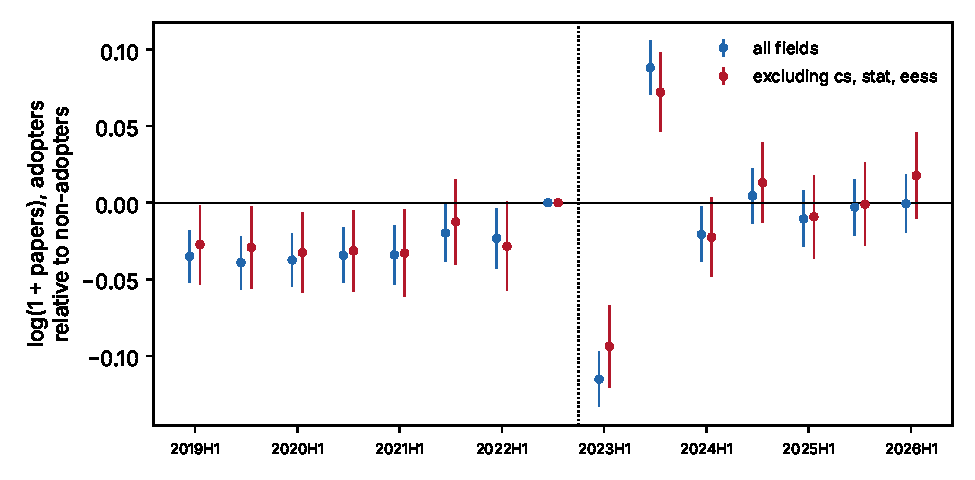
\includegraphics[width=0.75\textwidth]{figures/emp_llm_authors.pdf}
\caption{Author-level output of adopters of LLM-style writing, relative to
non-adopters (event study, reference 2022H2; 95\% intervals). Adoption is
classified from 2023 abstracts. Blue: all fields; red: excluding cs, stat and
eess.}
\label{fig:llm}
\end{figure}

\begin{figure}[t]
\centering
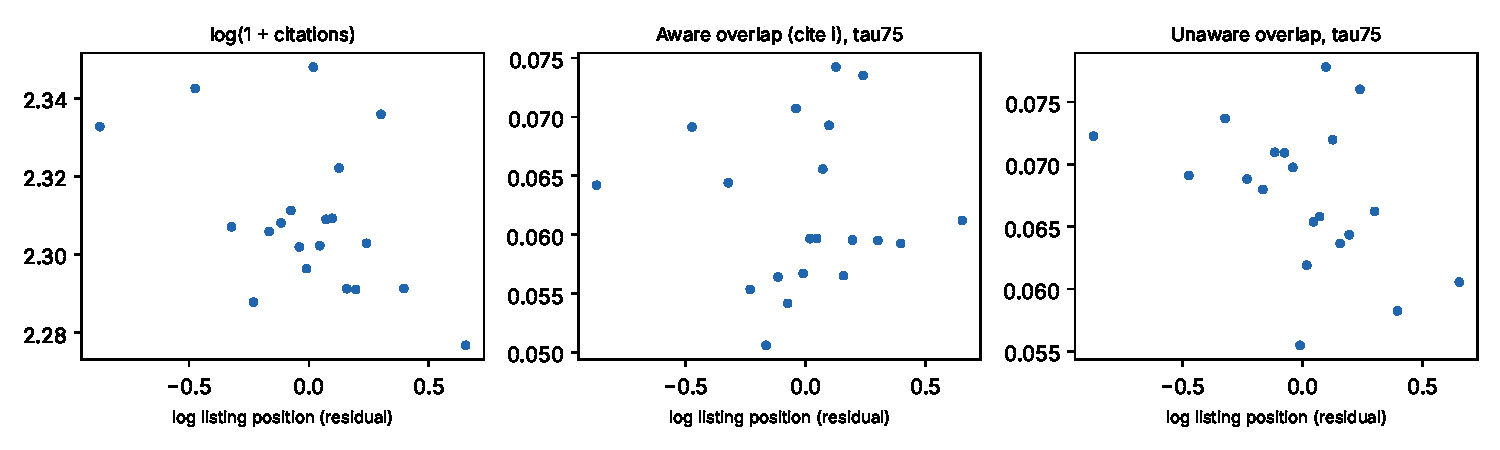
\includegraphics[width=\textwidth]{figures/emp_rank_design.pdf}
\caption{Listing rank in high-energy physics: binned residuals of outcomes on
residual log listing position (twenty bins), net of category-year and
submission-time fixed effects and log list size.}
\label{fig:rank}
\end{figure}


\end{document}
